% Options for packages loaded elsewhere
\PassOptionsToPackage{unicode}{hyperref}
\PassOptionsToPackage{hyphens}{url}
\PassOptionsToPackage{dvipsnames,svgnames*,x11names*}{xcolor}
%
\documentclass[
]{article}
\usepackage{lmodern}
\usepackage{amssymb,amsmath}
\usepackage{ifxetex,ifluatex}
\ifnum 0\ifxetex 1\fi\ifluatex 1\fi=0 % if pdftex
  \usepackage[T1]{fontenc}
  \usepackage[utf8]{inputenc}
  \usepackage{textcomp} % provide euro and other symbols
\else % if luatex or xetex
  \usepackage{unicode-math}
  \defaultfontfeatures{Scale=MatchLowercase}
  \defaultfontfeatures[\rmfamily]{Ligatures=TeX,Scale=1}
\fi
% Use upquote if available, for straight quotes in verbatim environments
\IfFileExists{upquote.sty}{\usepackage{upquote}}{}
\IfFileExists{microtype.sty}{% use microtype if available
  \usepackage[]{microtype}
  \UseMicrotypeSet[protrusion]{basicmath} % disable protrusion for tt fonts
}{}
\makeatletter
\@ifundefined{KOMAClassName}{% if non-KOMA class
  \IfFileExists{parskip.sty}{%
    \usepackage{parskip}
  }{% else
    \setlength{\parindent}{0pt}
    \setlength{\parskip}{6pt plus 2pt minus 1pt}}
}{% if KOMA class
  \KOMAoptions{parskip=half}}
\makeatother
\usepackage{xcolor}
\IfFileExists{xurl.sty}{\usepackage{xurl}}{} % add URL line breaks if available
\IfFileExists{bookmark.sty}{\usepackage{bookmark}}{\usepackage{hyperref}}
\hypersetup{
  colorlinks=true,
  linkcolor=blue,
  filecolor=Maroon,
  citecolor=Blue,
  urlcolor=blue,
  pdfcreator={LaTeX via pandoc}}
\urlstyle{same} % disable monospaced font for URLs
\usepackage[margin=1in]{geometry}
\usepackage{graphicx,grffile}
\makeatletter
\def\maxwidth{\ifdim\Gin@nat@width>\linewidth\linewidth\else\Gin@nat@width\fi}
\def\maxheight{\ifdim\Gin@nat@height>\textheight\textheight\else\Gin@nat@height\fi}
\makeatother
% Scale images if necessary, so that they will not overflow the page
% margins by default, and it is still possible to overwrite the defaults
% using explicit options in \includegraphics[width, height, ...]{}
\setkeys{Gin}{width=\maxwidth,height=\maxheight,keepaspectratio}
% Set default figure placement to htbp
\makeatletter
\def\fps@figure{htbp}
\makeatother
\setlength{\emergencystretch}{3em} % prevent overfull lines
\providecommand{\tightlist}{%
  \setlength{\itemsep}{0pt}\setlength{\parskip}{0pt}}
\setcounter{secnumdepth}{5}
\usepackage{titling}
\pretitle{\begin{center}\LARGE
\includegraphics[width=10cm]{input/images/facso.png}\\[\bigskipamount]}
\posttitle{\end{center}}
\usepackage{booktabs}
\usepackage{longtable}
\usepackage{array}
\usepackage{multirow}
\usepackage{wrapfig}
\usepackage{float}
\usepackage{colortbl}
\usepackage{pdflscape}
\usepackage{tabu}
\usepackage{threeparttable}
\usepackage{threeparttablex}
\usepackage[normalem]{ulem}
\usepackage{makecell}
\usepackage{xcolor}

\title{\vspace{5cm} Movilidad social subjetiva. Percepciones sobre ascenso,
descenso y permanencia en la escala de estatus social subjetivo en Chile}
\usepackage{etoolbox}
\makeatletter
\providecommand{\subtitle}[1]{% add subtitle to \maketitle
  \apptocmd{\@title}{\par {\large #1 \par}}{}{}
}
\makeatother
\subtitle{Curso Metodología I: Profesores Rodrigo Medel \& Nicolás Ratto -
Magíster en Ciencias Sociales mención Sociología de la Modernización}
\author{Kevin Carrasco Quintanilla}
\date{2021-07-10}

\begin{document}
\maketitle

\newpage

\hypertarget{introducciuxf3n.}{%
\section{Introducción.}\label{introducciuxf3n.}}

La igualdad de oportunidades es un pilar fundamental de las sociedades
democráticas modernas. Tanto así, que la Comisión económica para América
Latina y el Caribe (CEPAL) ha señalado que su importancia va más allá de
la estructura meritocrática de oportunidades (CEPAL,
\protect\hyperlink{ref-cepal_hora_2010}{2010}). Esto significa que las
democracias modernas deben garantizar a sus ciudadanos el derecho, ``por
el solo hecho de ser parte de la sociedad e independientemente de sus
logros individuales y recursos monetarios, a acceder a ciertos umbrales
de bienestar social y reconocimiento'' (CEPAL,
\protect\hyperlink{ref-cepal_hora_2010}{2010}, p. 11). En este sentido,
la igualdad de oportunidades es una situación ideal que garantiza un
mayor bienestar social y reconocimiento para cada uno de los ciudadanos,
donde las oportunidades ``no están predeterminadas por los recursos
económicos, sociales y culturales del hogar de origen, ni por
discriminaciones de género, raza, apariencia física o de otro tipo''
(PNUD, \protect\hyperlink{ref-pnud_Desiguales_2017}{2017}, p. 92). Sin
embargo, la desigualdad de oportunidades continúa siendo uno de los
temas principales en el debate público, tanto por sus consecuencias
materiales como por las distintas formas de legitimación social que
reproducen la desigualdad. Los índices de desigualdad (por ej.
Coeficiente Gini=0.44 en 2017) han posicionado a Chile como uno de los
países más desiguales de la región, donde incluso en la actualidad la
apariencia y el aspecto físico son un buen predictor de la clase social,
delatando ``a una sociedad con escasa movilidad social, en la que han
primado los prejuicios y la discriminación en el acceso a las
oportunidades'' (PNUD,
\protect\hyperlink{ref-pnud_Desiguales_2017}{2017}, p. 34).

Una de las principales herramientas para conocer las oportunidades que
una sociedad ofrece a sus ciudadanos consiste en establecer si un
individuo tendrá la posibilidad de lograr una mejoría en sus condiciones
de vida, sea durante su propia vida o con respecto a la situación de sus
padres (Espinoza et al.,
\protect\hyperlink{ref-espinoza_Estratificacion_2013}{2013}). Por lo
tanto, estudiar el grado de movilidad social que posee un país
constituye uno de los aspectos más relevantes para comprender el acceso
a oportunidades y a un mayor bienestar social por parte de los
individuos. Hasta ahora, los estudios sobre desigualdad y movilidad
social se han enfocado, por un lado, en los aspectos objetivos de la
movilidad, abarcando dimensiones sobre movilidad ocupacional a partir
del esquema de clases de Goldthorpe, Erikson y Portocarrero (EGP) (por
ej. Torche \& Wormald,
\protect\hyperlink{ref-torche_Estratificacion_2004}{2004}; Espinoza et
al., \protect\hyperlink{ref-espinoza_Estratificacion_2013}{2013}) y
sobre movilidad educacional, resaltando los beneficios que el ingreso a
la educación superior trae para sus integrantes (por ej. Pérez Verdugo,
\protect\hyperlink{ref-perezverdugo_Factores_2018}{2018}; PNUD,
\protect\hyperlink{ref-pnud_Desiguales_2017}{2017}). Por otro lado, un
poco menos estudiado han sido los aspectos subjetivos de la movilidad
social, que se refiere a las creencias subjetivas de los individuos con
respecto a su capacidad para ascender a una posición de clase social más
alta (Huang et al., \protect\hyperlink{ref-huang_Effects_2017}{2017}),
donde se han abarcado elementos como el estatus social subjetivo
(Castillo et al., \protect\hyperlink{ref-castillo_Todos_2013}{2013}) y
las percepciones y preferencias sobre la meritocracia y la desigualdad
económica (Castillo et al.,
\protect\hyperlink{ref-castillo_Meritocracia_2019}{2019}). Además, se ha
demostrado que una mayor movilidad social subjetiva está relacionada
positivamente con un mayor bienestar psicológico (Präg \& Gugushvili,
\protect\hyperlink{ref-prag_Subjective_2021}{2021}) y que altos niveles
de movilidad social subjetiva podrían actuar como un elemento
motivacional que alentara a los adolescentes a esforzarse para lograr
buenos resultados académicos (Zhang et al.,
\protect\hyperlink{ref-zhang_Family_2021}{2021}). De esta forma, el
objetivo de esta investigación es profundizar en la descripción de la
movilidad social subjetiva, abordando el estatus social subjetivo de los
individuos en comparación con el estatus social subjetivo de su familia
de procedencia y el estatus social subjetivo esperado para sus hijos.

Dentro de la movilidad social subjetiva se encuentran distintos
elementos que son determinantes para la percepción de los individuos
sobre las posibilidades que poseen para ascender en la escala de estatus
social. Estos elementos pueden ser tanto objetivos como subjetivos, ya
que la trayectoria de cada individuo puede ser explicada a partir de
propiedades personalmente adquiridas o por la pertenencia a un contexto
sociocultural o familiar determinado (Madero 2011, citado en Castillo et
al., \protect\hyperlink{ref-castillo_Todos_2013}{2013}, p. 160). Por un
lado, elementos objetivos como el nivel educacional, el nivel
socioeconómico y características adscriptivas como la raza o etnia
afectan directamente las percepciones que tienen los individuos sobre
sus propias oportunidades para ascender en una estructura meritocrática
de oportunidades ya que, por ejemplo, en los sectores populares se
tiende a poner la esperanza de movilidad social en las nuevas
generaciones, quienes al insertarse en el sistema de educación superior
serán ``más que uno'' (PNUD,
\protect\hyperlink{ref-pnud_Desiguales_2017}{2017}, p. 31). Por otro
lado, elementos como el estatus subjetivo de la familia de origen y el
estatus subjetivo esperado para sus hijos permiten explorar, por
ejemplo, en qué medida el posicionamiento de origen se asocia al
posicionamiento actual (Castillo et al.,
\protect\hyperlink{ref-castillo_Todos_2013}{2013}) y en qué medida la
diferencia entre el posicionamiento de origen y el posicionamiento
actual se asocia con el posicionamiento esperado para los hijos en la
escala de estatus social.

De esta forma, el presente estudio se guía a partir de las preguntas
sobre ¿cuál es el grado de movilidad social subjetiva percibida en
Chile? Y, considerando la importancia de factores objetivos y
subjetivos, ¿cuál es la relación del nivel educacional y la percepción
de meritocracia con el grado de movilidad social subjetiva? Así, se
espera contribuir en una mayor comprensión del nivel de movilidad social
percibido por la sociedad chilena a partir de distintos elementos que
podrían afectar la percepción de la movilidad experimentada y esperada
en la escala de estatus social.

\hypertarget{objetivo-general}{%
\section{Objetivo general}\label{objetivo-general}}

Debido a que esta investigación busca, en primer lugar, describir la
percepción de movilidad social subjetiva en Chile y, en segundo lugar,
analizar la asociación entre factores objetivos y subjetivos sobre la
percepción de movilidad social subjetiva, se plantea esta investigación
bajo un carácter descriptivo y correlacional. De esta forma, se plantea
el siguiente objetivo: Describir el nivel de movilidad social subjetiva
en Chile durante el 2019 y su asociación con dos elementos que podrían
condicionar la percepción de movilidad social subjetiva, la que permite
percibir el ascenso, descenso o permanencia experimentada y esperada en
la escala de estatus social.

\hypertarget{objetivos-especuxedficos}{%
\subsection{Objetivos específicos}\label{objetivos-especuxedficos}}

\begin{enumerate}
\def\labelenumi{\arabic{enumi}.}
\item
  Describir la percepción de movilidad social subjetiva experimentada en
  Chile durante el 2019 a partir de la diferencia entre el estatus
  social subjetivo individual y el estatus social subjetivo de la
  familia de procedencia.
\item
  Describir la percepción de movilidad social subjetiva esperada en
  Chile durante el 2019 a partir de la diferencia entre el estatus
  social subjetivo esperado para los hijos y el estatus social subjetivo
  individual.
\item
  Analizar si la experiencia de movilidad social ascendente se asocia
  con un mayor nivel de movilidad social esperada para los hijos.
\item
  Analizar si dos elementos, uno objetivo (nivel educacional del
  entrevistado) y otro subjetivo (percepción de meritocracia), se
  asocian con la percepción de movilidad social experimentada y esperada
  en Chile durante el 2019.
\end{enumerate}

\hypertarget{antecedentes}{%
\section{Antecedentes}\label{antecedentes}}

La movilidad social intergeneracional se refiere a las diferencias en
las desigualdades sociales y su transmisión entre padres e hijos, donde
una baja movilidad intergeneracional indica que la posición social de
las personas se ve determinada por la posición social de sus padres,
mientras que una alta movilidad intergeneracional indica una relativa
independencia entre la posición social de padres e hijos (PNUD,
\protect\hyperlink{ref-pnud_Desiguales_2017}{2017}, p. 74). En este
sentido, existen diferentes formas de comparar la posición social entre
padres e hijos, siendo uno de los principales la que respecta al enfoque
de la movilidad ocupacional, donde Torche \& Wormald
(\protect\hyperlink{ref-torche_Estratificacion_2004}{2004}) señalan que
en Chile existe una mayor movilidad relativa en la parte baja de la
pirámide social, asociada a los movimientos de salida y entrada de la
pobreza. Por el contrario, Ruiz \& Boccardo
(\protect\hyperlink{ref-ruiz_chilenos_2014}{2014}) señalan una
dificultad para continuar con el enfoque tradicional de movilidad social
bajo una perspectiva ocupacional, ya que a partir de las nuevas
condiciones laborales marcadas principalmente por la precarización y el
subcontrato, se modifica el proceso actual de formación de clases
sociales. Por su parte, Espinoza, et. al
(\protect\hyperlink{ref-espinoza_Estratificacion_2013}{2013}) señalan
que resulta más difícil en 2009 que en 1999 encontrarse en una clase
ocupacional sustantivamente diferente a la de los padres. Esto implica
que en Chile existe ``una estructura de clases relativamente móvil y
permeable en su parte media, pero que presenta una tendencia a la
polarización, pues las distancias sociales continúan aumentando a pesar
del crecimiento económico'' (Espinoza et al.,
\protect\hyperlink{ref-espinoza_Estratificacion_2013}{2013}, p. 187). En
este sentido, cuando las personas comparan su posición actual con la de
generaciones anteriores existe cierto grado de acuerdo sobre los
progresos del país, pero predomina una sensación de que la movilidad
sigue siendo relativa, de que los grupos altos siguen teniendo
seguridades y ventajas que el resto no tiene (PNUD,
\protect\hyperlink{ref-pnud_Desiguales_2017}{2017}, p. 163).

Otra forma de comparar la posición social entre padres e hijos emerge
desde la necesidad de explorar nuevas fuentes de información que
permitan comprender el nivel de movilidad social que posee una sociedad,
a fin de conocer cuáles son las percepciones que poseen las personas a
pesar de los avances y reconocimientos de una movilidad social objetiva.
Abordar esta dimensión de percepciones sobre movilidad social implica
enfocarse en lo que es observado por los individuos y las consecuencias
que esto tiene para la sociedad. Específicamente, la hipótesis de una
perspectiva de movilidad ascendente (\emph{the POUM hypothesis}) implica
que los individuos que están por debajo del promedio de ingresos son
optimistas sobre su futuro, tanto propio como el de sus hijos, y que,
debido a este optimismo, estarían menos de acuerdo con políticas
redistributivas, ya que estas podrían perjudicarlos en el futuro
(Benabou \& Ok, \protect\hyperlink{ref-benabou_Social_1998}{1998}). Sin
embargo, Gavira (\protect\hyperlink{ref-gavira_Social_2008}{2008})
señala que en América Latina la mayor parte de la población (47\%)
percibe que se encuentra en la misma posición que sus padres, mientras
que un 33\% cree que se encuentra más abajo que sus padres y solo un
20\% percibe que se encuentra por sobre el estatus social de sus padres.

Para el caso chileno, una de las principales investigaciones realizadas
bajo esta línea de investigación es la llevada a cabo por Castillo, et.
al (\protect\hyperlink{ref-castillo_Todos_2013}{2013}), donde se señala
que el estatus social subjetivo de la familia de procedencia influye
positivamente en el estatus social subjetivo individual, excepto en el
nivel más alto de la escala de estatus social subjetivo familiar, donde
los individuos tienden a ubicarse en posiciones más bajas de la escala.
De esta forma, considerando la evidencia previa y que, en general, se
percibe un mayor crecimiento económico, se plantea la siguiente
hipótesis:

\begin{quote}
\textbf{\emph{H1}}: Los individuos se ubican en una posición mayor de la
escala de estatus social subjetivo que la posición en que ubican a sus
familias de procedencia. Es decir, las diferencias entre el estatus
social subjetivo individual y el familiar serán en su mayoría positivas.
(Percepción ascendente de movilidad experimentada)
\end{quote}

\begin{quote}
\textbf{\emph{H2}}: Los individuos ubicarán a sus hijos en una posición
mayor de la escala de estatus social subjetivo que la posición en que se
ubican a sí mismos. Es decir, las diferencias entre el estatus social
subjetivo esperado para sus hijos y el estatus propio serán en su
mayoría positivas. (Percepción ascendente de movilidad esperada)
\end{quote}

De manera similar a lo anterior, Pérez Verdugo
(\protect\hyperlink{ref-perezverdugo_Factores_2018}{2018}) señala que
quienes poseen experiencias individuales positivas en torno a la
movilidad social suelen aprender cuales son los factores que influyen en
el éxito económico, afectando directamente a sus acciones futuras. Así,
se plantea la siguiente hipótesis sobre el estatus social esperado para
los hijos:

\begin{quote}
\textbf{\emph{H3}}: Un mayor grado de movilidad social experimentada se
asocia con un mayor grado de movilidad social esperada, es decir, los
individuos que perciben que han experimentado una movilidad social
ascendente esperan que sus hijos también experimenten una movilidad
social ascendente
\end{quote}

Asimismo, Castillo, et. al
(\protect\hyperlink{ref-castillo_Educacion_2013}{2013}) señalan que la
percepción de desigualdad no es un espejo de la realidad, sino que se
producen una serie de sesgos relacionados con dos fuentes: el origen
social (por ejemplo, la clase social o el estatus) y las creencias
culturales que predominan acerca de la justicia distributiva y la
meritocracia. En este sentido, la educación, en la medida que juega un
papel importante en la determinación de la condición social de las
personas, es apreciada como canal de movilidad social (Ruiz \& Boccardo,
\protect\hyperlink{ref-ruiz_chilenos_2014}{2014}, p. 60). Por lo tanto,
se propone evaluar dos aspectos que podrían estar asociados con la
percepción de movilidad social experimentada y esperada, a saber, el
nivel educacional del entrevistado y la percepción de meritocracia.

\begin{quote}
\textbf{\emph{H4.1}}: Individuos que poseen un mayor nivel educacional
perciben que han experimentado una mayor movilidad social subjetiva y
esperan que sus hijos también experimenten una movilidad social
subjetiva ascendente.
\end{quote}

\begin{quote}
\textbf{\emph{H4.2}}: Individuos que perciben un mayor nivel de
meritocracia en el país perciben que han experimentado una mayor
movilidad social subjetiva y esperan que sus hijos también experimenten
una movilidad social subjetiva ascendente.
\end{quote}

\hypertarget{metodologuxeda}{%
\section{Metodología}\label{metodologuxeda}}

La metodología planteada para realizar esta investigación es de carácter
cuantitativa a partir de datos secundarios. Más precisamente, el Centro
de Estudios de Conflicto y Cohesión Social (COES) realiza desde el año
2016 el primer ``Estudio Longitudinal Social de Chile'' (ELSOC). Este
estudio consiste en encuestar a casi 3.000 chilenos, anualmente, a lo
largo de una década. Por lo tanto, el diseño de ELSOC es cuantitativo de
tipo panel, es decir, que se repite su aplicación año a año.

El principal objetivo de ELSOC es evaluar la manera como piensan,
sienten y se comportan los chilenos en torno a un conjunto de temas
referidos al conflicto y la cohesión social en Chile. Además, permite
comparar la estabilidad o cambio en diversas dimensiones sociales
atendiendo a factores que los moderan o explican a lo largo de los años
(COES, \protect\hyperlink{ref-coes_Estudio_2021}{2021}).

Esta encuesta es aplicada por medio de un cuestionario estructurado que
posee 7 módulos diferentes: Territorio, Redes y actitudes sociales,
Ciudadanía y democracia, Desigualdad y legitimidad, Conflicto social,
Salud y bienestar y Caracterización sociodemográfica. Posee un muestreo
probabilístico, estratificado (por tamaño de ciudades), por
conglomerados y multietápico (aleatorio en todas sus etapas): Se
eligieron aleatoriamente 40 ciudades con más de 10.000 habitantes (92
comunas de 13 regiones), dentro de estas se escogieron aleatoriamente
1067 manzanas. Dentro de cada manzana se escogieron hogares
aleatoriamente y dentro de cada hogar fueron elegidos aleatoriamente
individuos con 18 años o más. Por lo tanto, su unidad básica de
observación son personas individuales. Asimismo, la población objetivo
son hombres y mujeres de 18 a 75 años. Esta encuesta alcanza un 77\% de
representatividad de la población total del país y un 93\% de la
población urbana, con un error muestral del 2\%. La muestra alcanzada en
2019 posee las respuestas de 3417 individuos, que incluye respuestas de
participantes de la primera ola (2016) y de la muestra de refresco
iniciada en 2018 (COES,
\protect\hyperlink{ref-coes_Radiografia_2019}{2019}).

En lo específico de esta investigación, se propone realizar un análisis
univariado que permita describir la variación de las variables
dependientes para, posteriormente, realizar un análisis bivariado con el
fin de ver si esta variación de las variables dependientes se asocia con
las variables independientes.

\hypertarget{mediciuxf3n-y-operacionalizaciuxf3n-de-variables}{%
\subsection{Medición y operacionalización de
variables}\label{mediciuxf3n-y-operacionalizaciuxf3n-de-variables}}

En ELSOC, dentro de su módulo de Desigualdad y Legitimidad, se incluyen
tres preguntas que abordan el estatus social subjetivo de las personas:
(1) El estatus social subjetivo del entrevistado; (2) el estatus social
subjetivo en que ubica a su familia de procedencia; y (3) el estatus
social subjetivo en que el entrevistado cree que se ubicarán sus hijos.

\begin{table}[!h]

\caption{\label{tab:unnamed-chunk-3}Estatus social subjetivo}
\centering
\fontsize{8}{10}\selectfont
\begin{tabu} to \linewidth {>{\raggedright\arraybackslash}p{2 cm}>{\raggedright\arraybackslash}p{4 cm}>{\raggedright\arraybackslash}p{3 cm}>{\raggedright\arraybackslash}p{4 cm}}
\toprule
Dimensión & Encabezado & Categoría de respuesta & Indicador\\
\midrule
 &  &  & ¿Dónde se ubicaría usted en la sociedad chilena?\\
\cmidrule{4-4}
 &  &  & Y pensando en la familia en la que usted creció, ¿dónde se ubicarían ellos en esta escala?\\
\cmidrule{4-4}
\multirow{-3}{2 cm}{\raggedright\arraybackslash Estatus social subjetivo} & \multirow{-3}{4 cm}{\raggedright\arraybackslash En nuestra sociedad, hay grupos que tienden a ubicarse en los niveles más altos y grupos que tienden a ubicarse en los niveles más bajos de la sociedad.} & \multirow{-3}{3 cm}{\raggedright\arraybackslash Escala de 0 a 10. 0 El nivel mas bajo y 10 El nivel mas alto} & Si usted tiene actualmente hijos o si los tuviera en el futuro, ¿dónde cree usted que se ubicarían ellos?\\
\bottomrule
\end{tabu}
\end{table}

A partir de estos tres indicadores que se presentan en la tabla 1 se
construirán dos variables dependientes que miden Movilidad Social
Subjetiva. Siguiendo el trabajo de (Gavira,
\protect\hyperlink{ref-gavira_Social_2008}{2008}), por un lado, se
medirá la percepción de movilidad social subjetiva experimentada por los
encuestados a partir de la diferencia entre su estatus social subjetivo
y el estatus social subjetivo en que ubica a su familia de procedencia.
Por otro lado, se medirá la percepción de movilidad social subjetiva
esperada a partir de la diferencia entre el estatus social subjetivo
esperado para sus hijos y el estatus social subjetivo de los
encuestados. De esta forma, valores negativos de estas variables indican
una movilidad social subjetiva descendente, valores positivos indican
una movilidad social subjetiva ascendente y el valor 0 indica que los
individuos no perciben movilidad social.

En relación con las variables independientes, estas pretenden ver la
asociación que existe entre un factor objetivo y otro subjetivo sobre
las variables dependientes. Por lo tanto, se utilizará el nivel
educacional de los encuestados como una factor objetivo y el grado de
percepción de meritocracia como un factor subjetivo. Estas variables se
presentan en su versión original en la tabla 2. De esta forma, el nivel
educacional fue agrupado en 4 categorías: 1) Educación básica o menos;
2) Educación media; 3) Educación técnica superior; y 4) Educación
universitaria y postgrado. Asimismo, la percepción de meritocracia será
medida a partir de un índice promedio entre dos variables: 1) el grado
de acuerdo con que el esfuerzo es recompensado; y 2) el grado de acuerdo
con que la inteligencia es recompensada.

\begin{table}[!h]

\caption{\label{tab:unnamed-chunk-5}Variables independientes}
\centering
\fontsize{8}{10}\selectfont
\begin{tabu} to \linewidth {>{\raggedright\arraybackslash}p{2 cm}>{\raggedright\arraybackslash}p{4 cm}>{\raggedright\arraybackslash}p{4 cm}>{\raggedright\arraybackslash}p{4 cm}}
\toprule
Dimensión & Encabezado & Indicador & Categoría de respuesta\\
\midrule
 &  &  & Totalmente en desacuerdo\\
\cmidrule{4-4}
 &  &  & En desacuerdo\\
\cmidrule{4-4}
 &  &  & Ni en desacuerdo ni de acuerdo\\
\cmidrule{4-4}
 &  &  & De acuerdo\\
\cmidrule{4-4}
 &  & \multirow{-5}{4 cm}{\raggedright\arraybackslash En Chile las personas son recompensadas por sus esfuerzos} & Totalmente de acuerdo\\
\cmidrule{3-4}
 &  &  & Totalmente en desacuerdo\\
\cmidrule{4-4}
 &  &  & En desacuerdo\\
\cmidrule{4-4}
 &  &  & Ni en desacuerdo ni de acuerdo\\
\cmidrule{4-4}
 &  &  & De acuerdo\\
\cmidrule{4-4}
\multirow{-10}{2 cm}{\raggedright\arraybackslash Percepción de meritocracia} & \multirow{-10}{4 cm}{\raggedright\arraybackslash ¿En qué medida se encuentra usted de acuerdo o en desacuerdo con cada una de las siguientes afirmaciones?} & \multirow{-5}{4 cm}{\raggedright\arraybackslash En Chile las personas son recompensadas por su inteligencia y habilidades} & Totalmente de acuerdo\\
\cmidrule{1-4}
 &  &  & Educación básica o menos\\
\cmidrule{4-4}
 &  &  & Educación media\\
\cmidrule{4-4}
 &  &  & Educación técnica profesional\\
\cmidrule{4-4}
\multirow{-4}{2 cm}{\raggedright\arraybackslash Nivel educacional} & \multirow{-4}{4 cm}{\raggedright\arraybackslash ¿Cuál es su nivel educacional? Indique el tipo de estudio actual (si estudia actualmente) o el último tipo aprobado (si no estudia actualmente).} & \multirow{-4}{4 cm}{\raggedright\arraybackslash } & Educación superior o postgrado\\
\bottomrule
\end{tabu}
\end{table}

\hypertarget{anuxe1lisis-descriptivo}{%
\section{Análisis descriptivo}\label{anuxe1lisis-descriptivo}}

\begin{figure}

{\centering 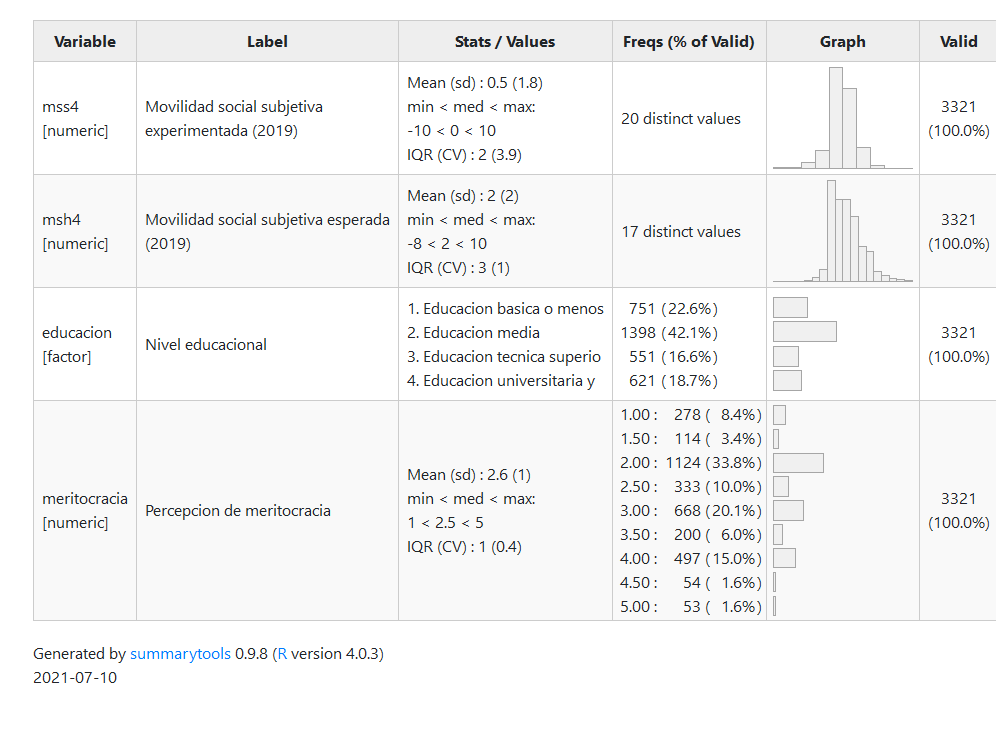
\includegraphics[width=1\linewidth,height=1\textheight]{output/tables/table1} 

}

\caption{Tabla de descriptivos}\label{fig:unnamed-chunk-6}
\end{figure}

La muestra final utilizada en este estudio es de 3321 casos (NA=96). En
la figura 1 se presentan los principales descriptivos de las variables
utilizadas. De manera general, es posible señalar que la movilidad
social subjetiva experimentada posee valores entre -10 y 10, con una
mediana de 0 y una media de 0,5 (sd=1.8), mientras que la movilidad
social subjetiva esperada posee valores entre -8 y 10, con una mediana
de 2 y una media de 2 (sd=2). En cuanto a las variables independientes,
la mayor parte de la muestra posee educación media (42.1\%), mientras
que la percepción de meritocracia posee valores entre 1 y 5, con una
mediana de 2.5 y una media de 2.6 (sd=1).

\begin{figure}

{\centering 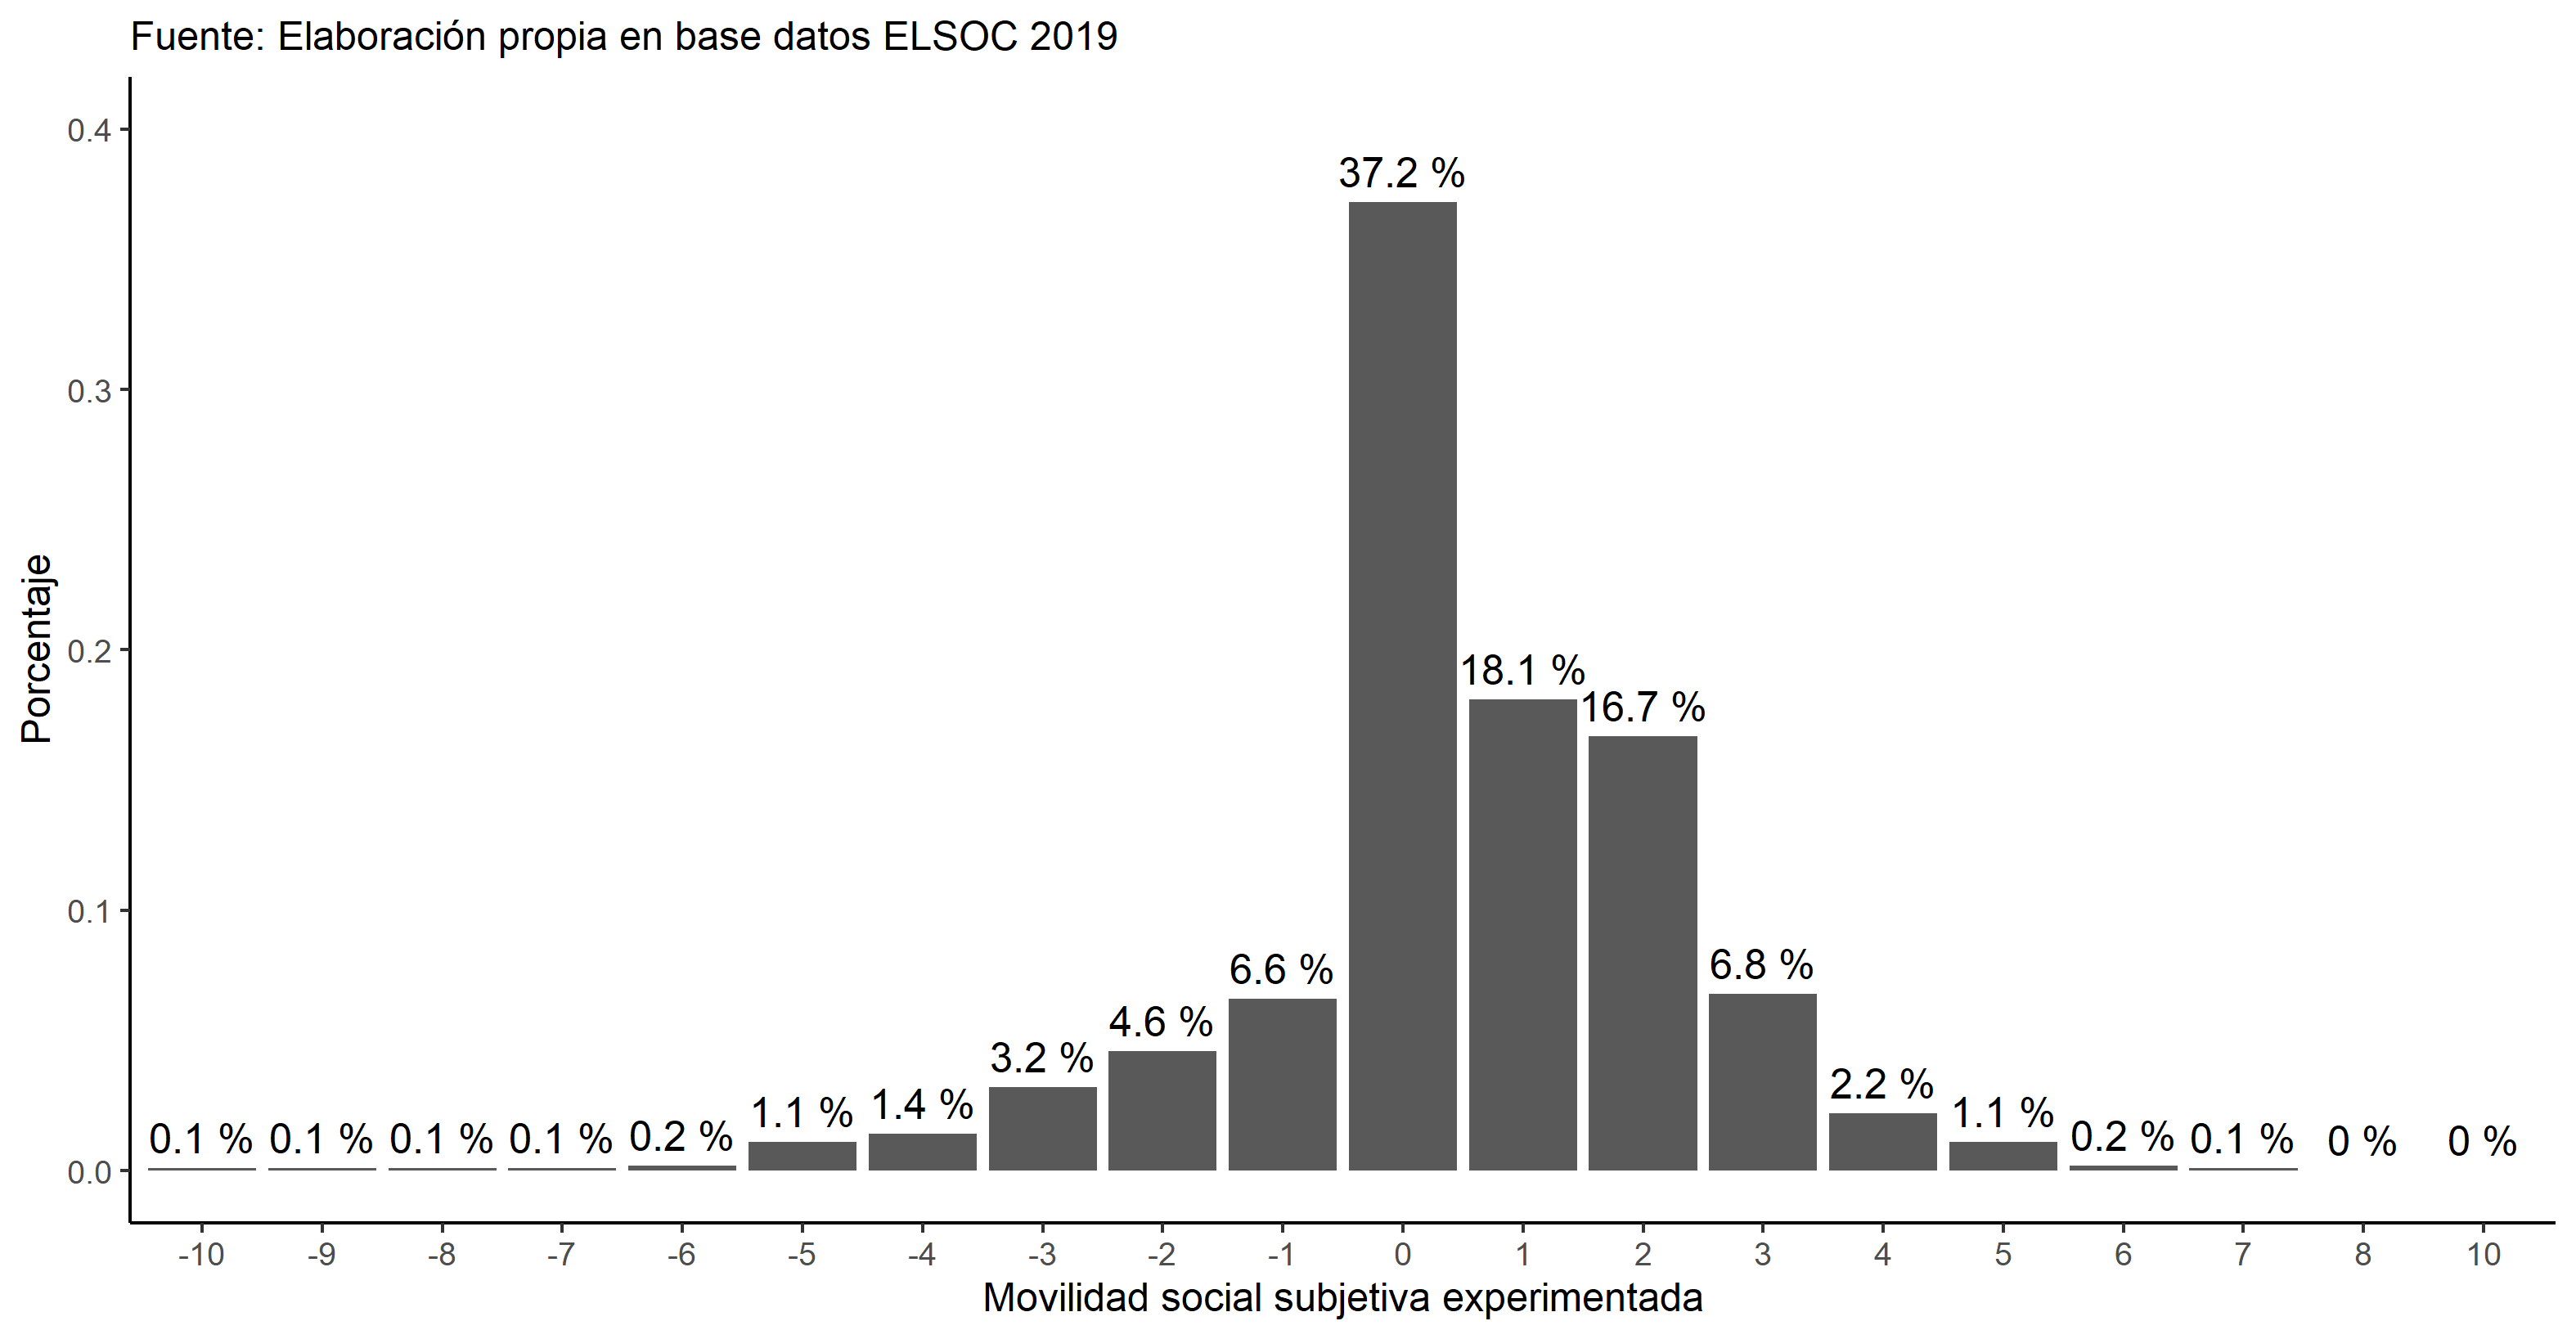
\includegraphics[width=0.8\linewidth,height=0.8\textheight]{output/graphs/graf1} 

}

\caption{Movilidad social subjetiva experimentada (muestra)}\label{fig:unnamed-chunk-7}
\end{figure}

En la figura 2 se presenta la percepción de movilidad social subjetiva
experimentada, es decir, el grado en que los individuos perciben que se
han movido en la escala de estatus social subjetivo en comparación con
el estatus de sus padres. Así, se puede observar que una gran parte de
la muestra percibe una ausencia de movilidad social subjetiva (37.2\%),
un 45.2\% percibe que se encuentra en, al menos, una posición superior a
la posición que ocupaban sus padres (un 18.1\% en una posición sobre la
de sus padres y un 0.1\% siete posiciones sobre sus padres) y un 17.5\%
percibe que se encuentra en, por lo menos, una posición inferior a la
posición que ocupaban sus padres (un 6.6\% una posición bajo la de sus
padres y un 0.1\% diez posiciones bajo sus padres). En resumen, los
individuos perciben que su posición no ha cambiado radicalmente en
comparación con sus padres, lo que va en línea con la literatura previa:
En la escala de estatus social subjetivo se perciben bajas
probabilidades de experimentar una movilidad social ascendente o
descendente, demostrando que se percibe una estructura social más bien
rígida.

\begin{figure}

{\centering 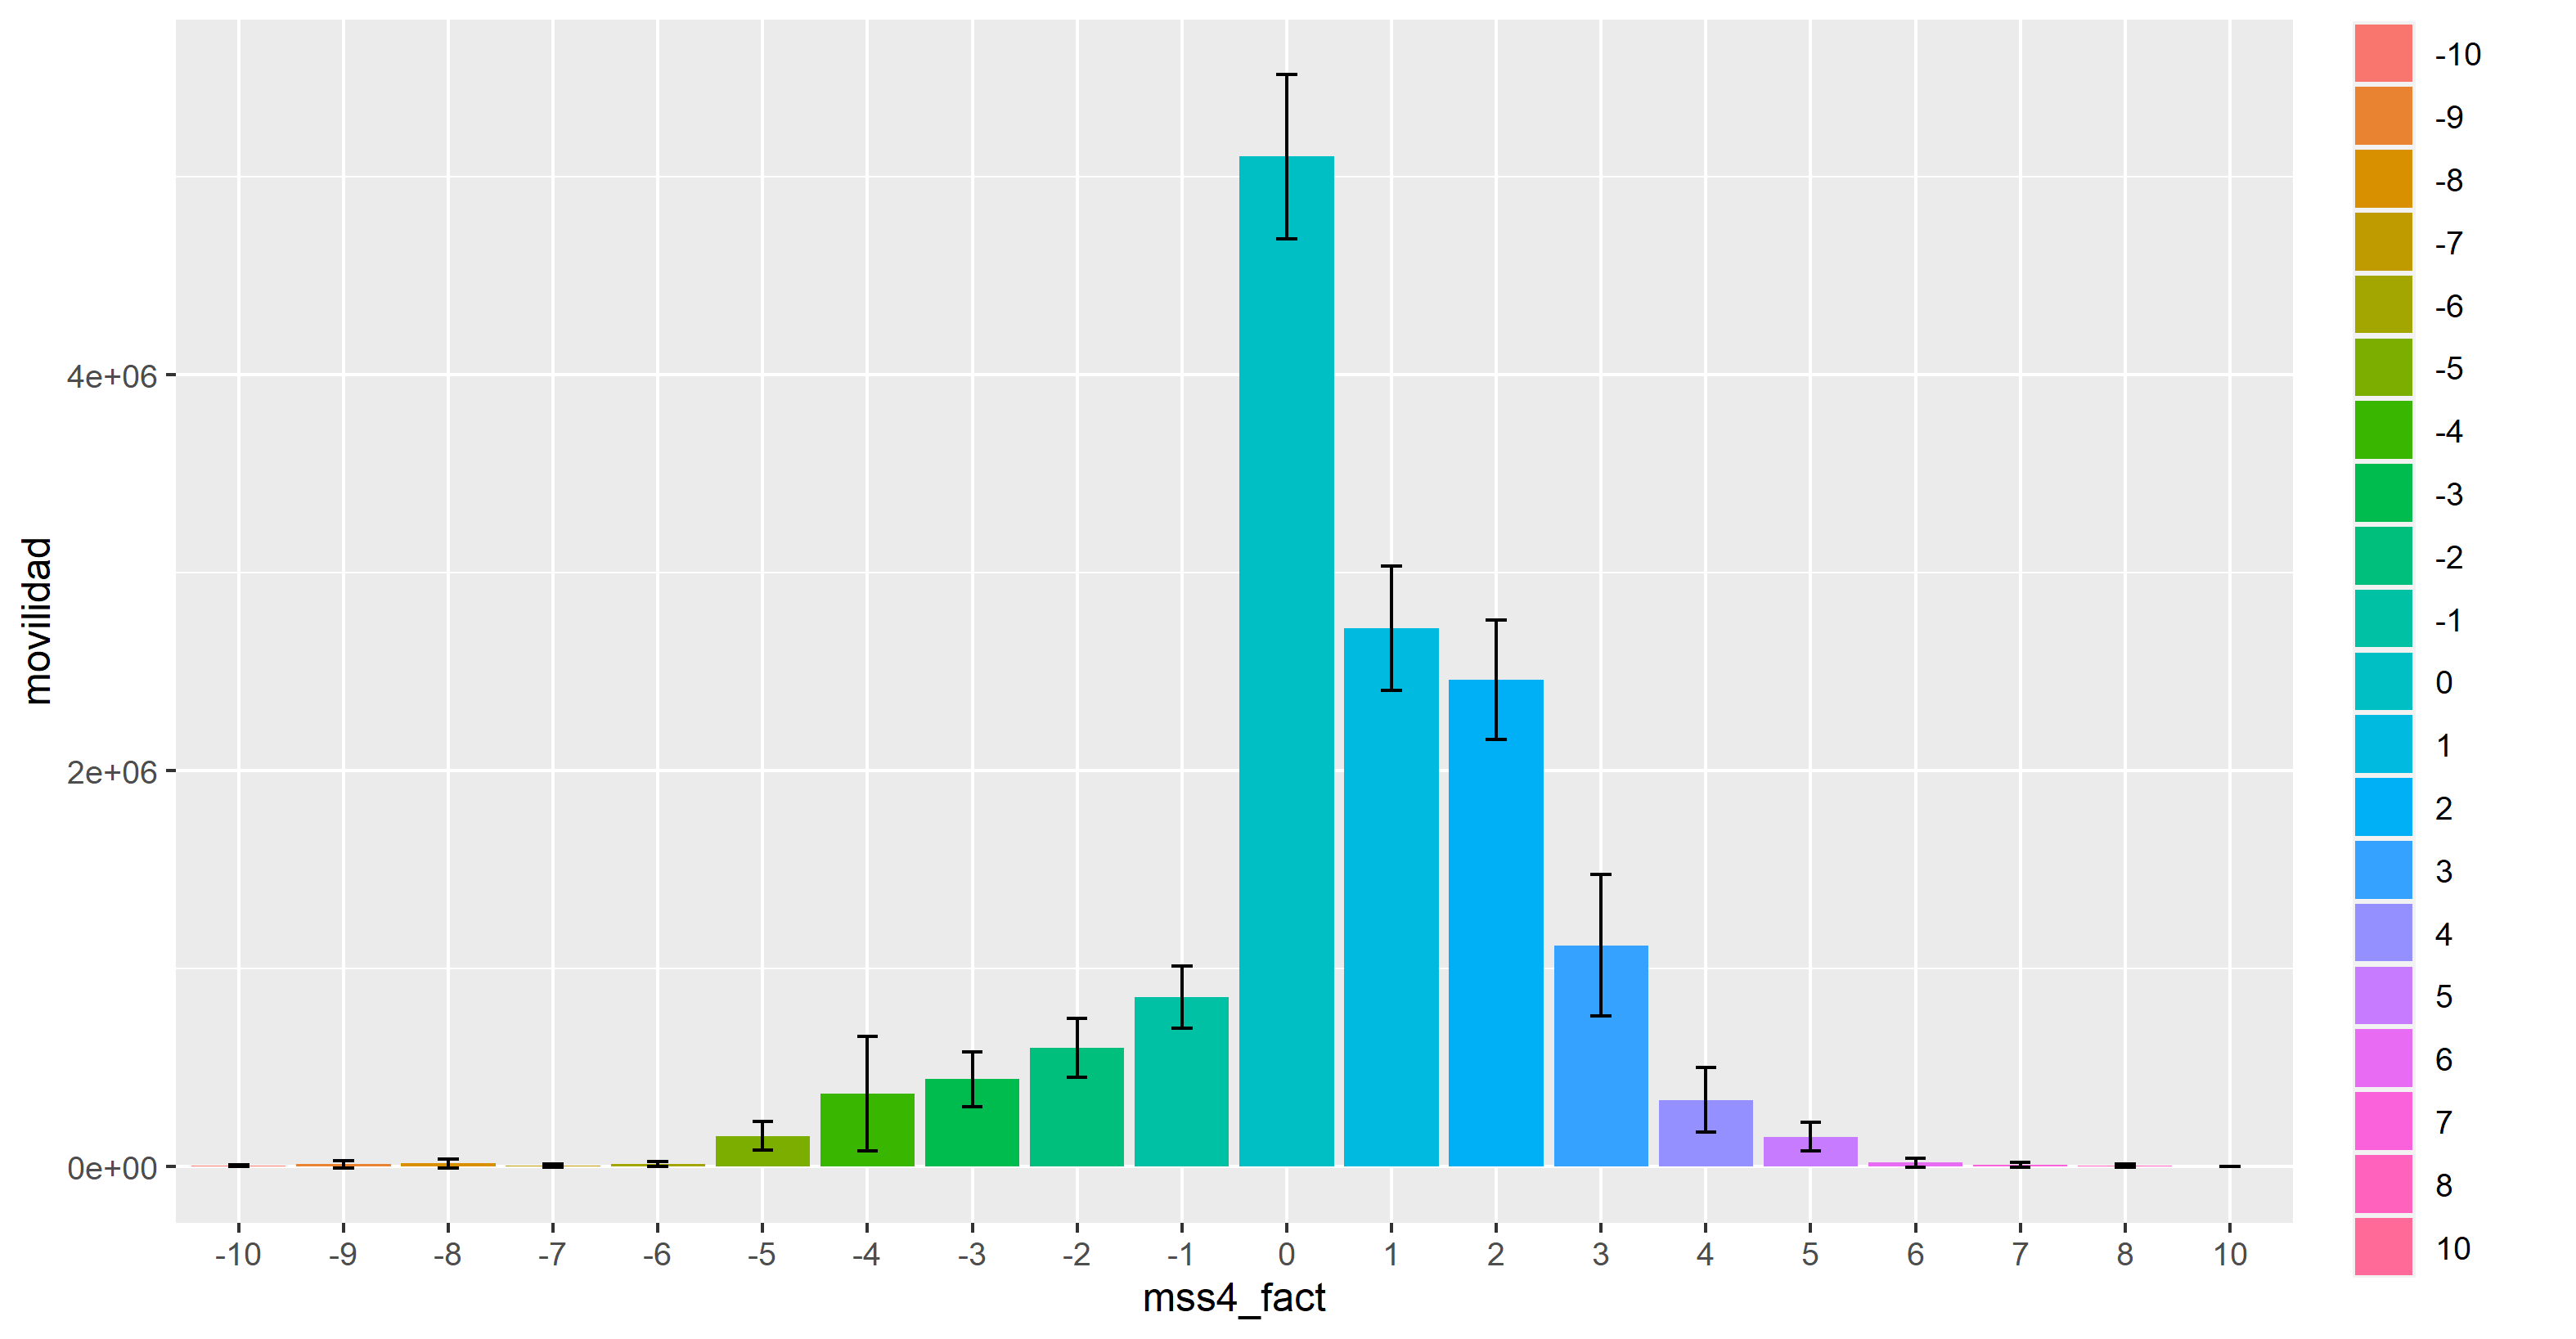
\includegraphics[width=0.8\linewidth,height=0.8\textheight]{output/graphs/graf1_exp} 

}

\caption{Movilidad social subjetiva experimentada (población)}\label{fig:unnamed-chunk-8}
\end{figure}

Como se muestra en la figura 3, estos resultados son extrapolables a la
población. En este sentido, más de cinco millones de habitantes perciben
que se encuentran en la misma posición de la escala de estatus social
subjetivo que sus padres, mientras que un aproximado de dos a tres
millones de habitantes perciben que están una o dos posiciones arriba de
sus padres (no hay diferencias significativas entre estos dos grupos).
Finalmente, un aproximado de tres millones de personas perciben que se
encuentran más abajo en la escala de estatus social subjetivo que sus
padres.

\begin{figure}

{\centering 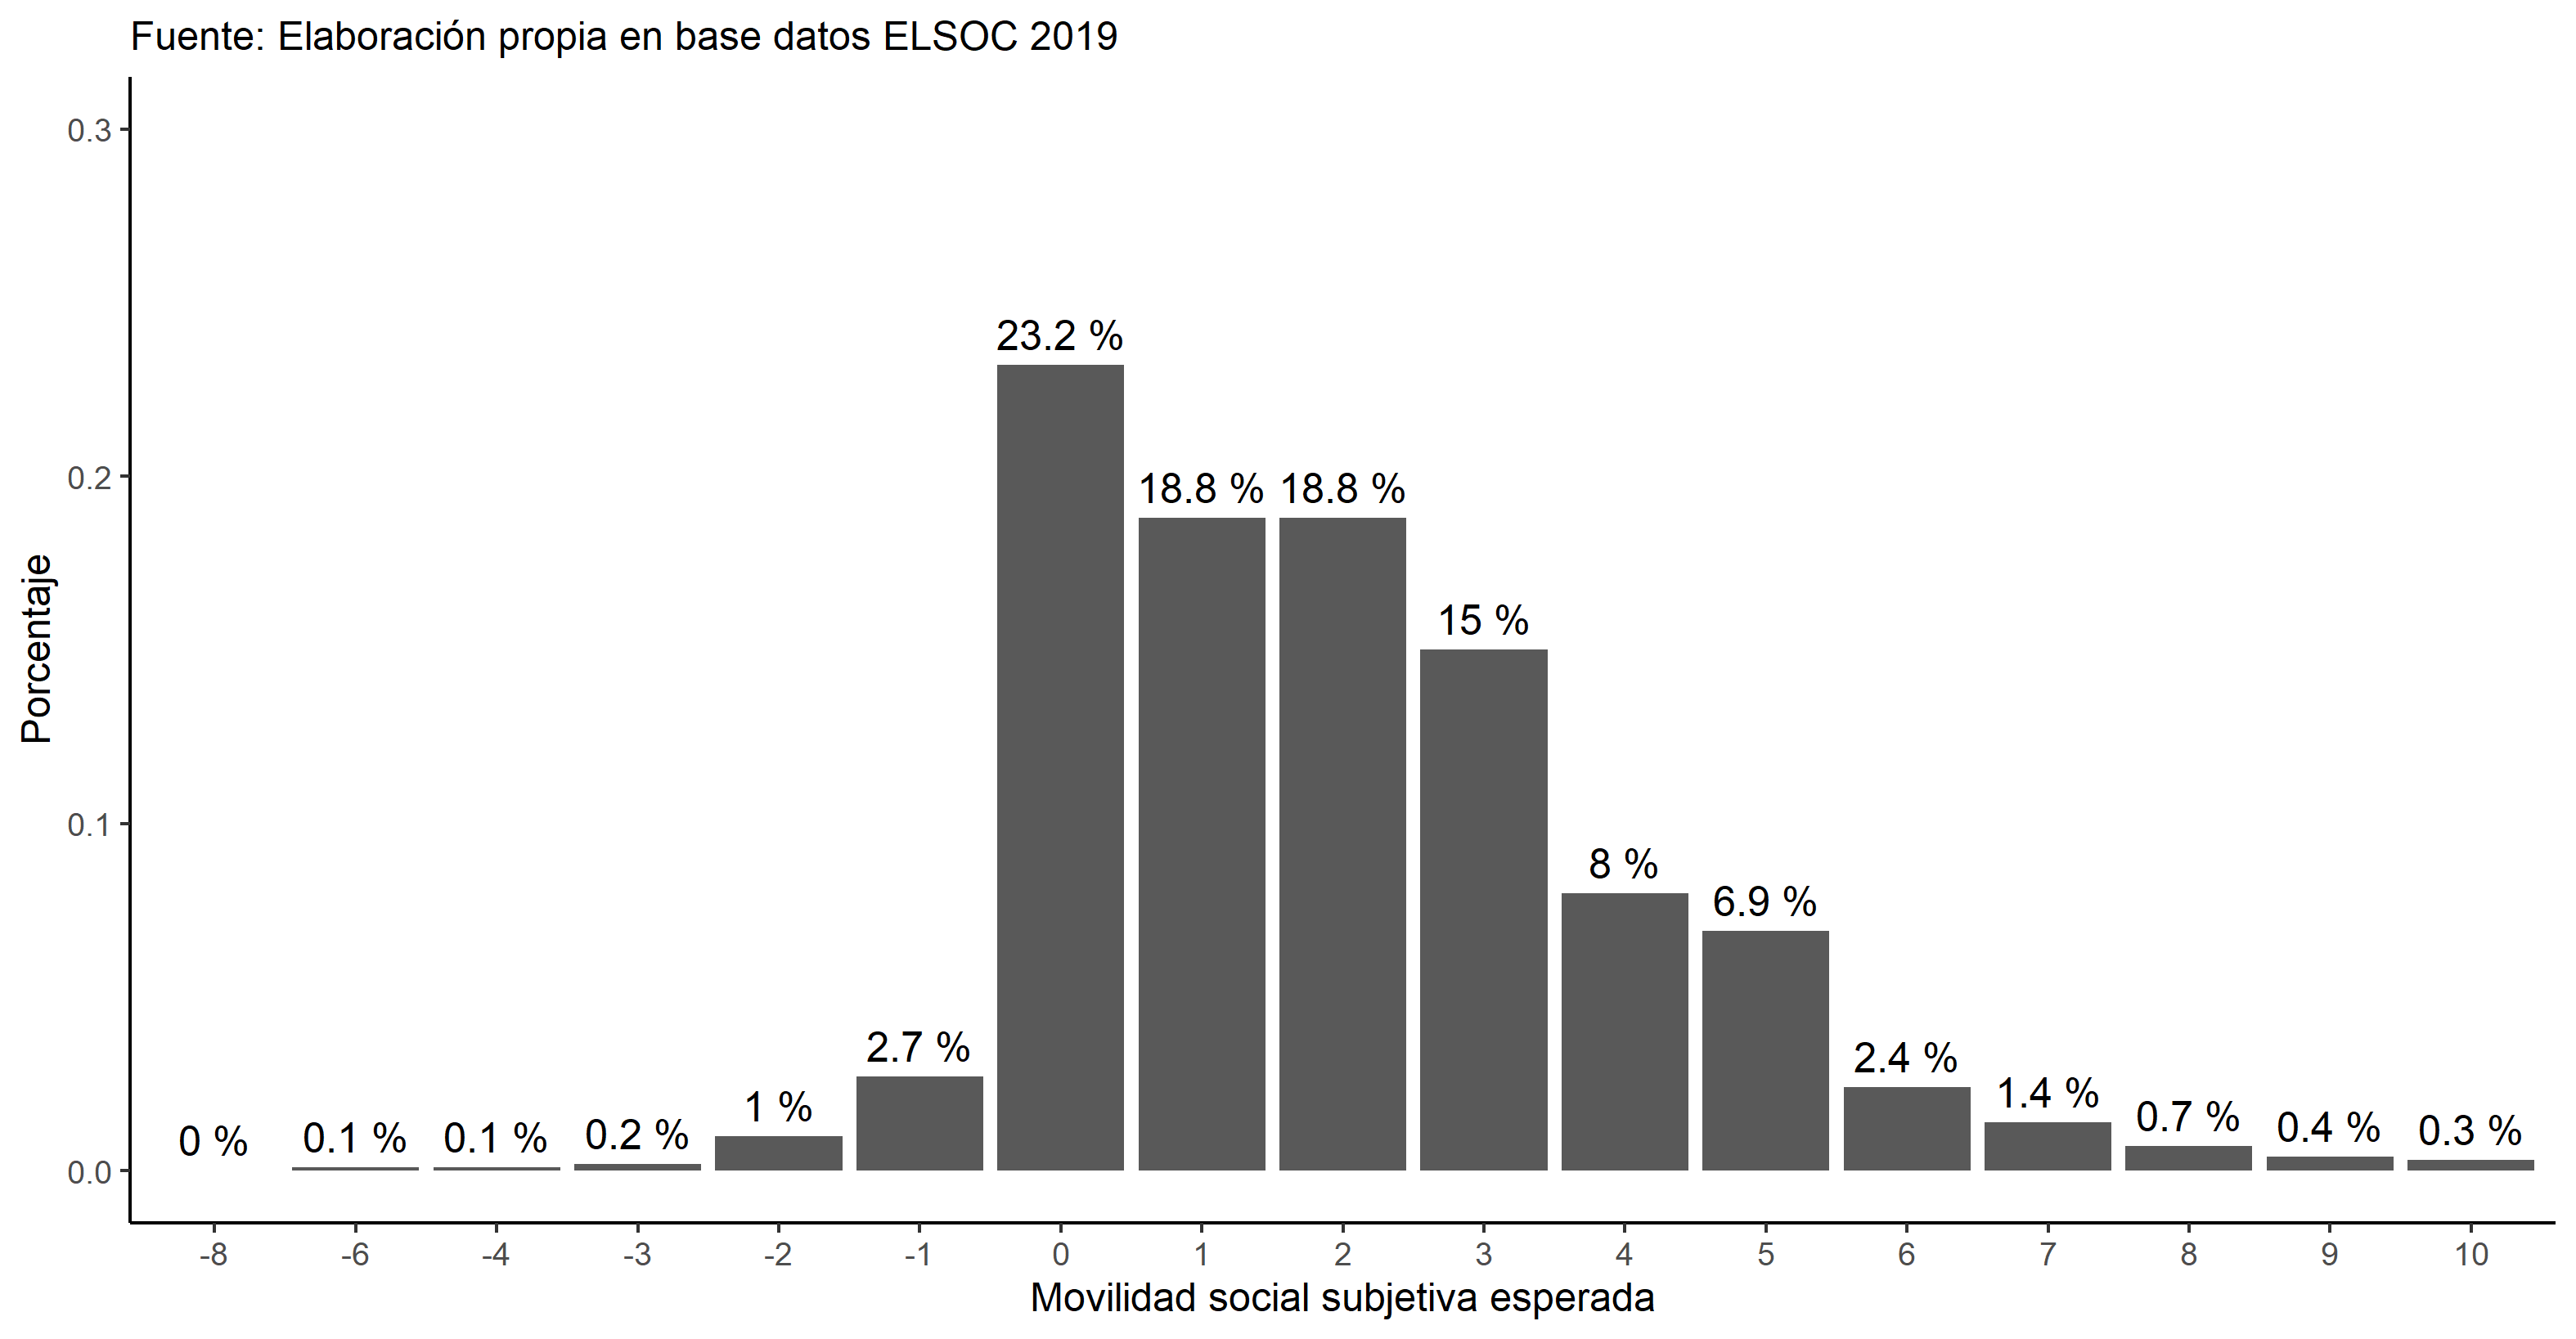
\includegraphics[width=0.8\linewidth,height=0.8\textheight]{output/graphs/graf2} 

}

\caption{Movilidad social subjetiva esperada (muestra)}\label{fig:unnamed-chunk-9}
\end{figure}

En la figura 4 se presenta la percepción de movilidad social subjetiva
esperada, es decir, el grado en que los individuos perciben que sus
hijos podrán ascender o descender dentro de la estructura de estatus
social en comparación con su posición actual. De esta forma, se puede
observar que un 23.2\% de la muestra percibe que sus hijos se
encontrarán en la misma posición de estatus social en la que ellos se
encuentran actualmente, un 72.7\% percibe que sus hijos se encontrarán
en una posición superior a la de ellos (un 18.8\% percibe que se
encontrarán una posición más arriba y un 0.3\% que se encontrarán diez
posiciones más arriba) y un 4.1\% percibe que sus hijos se encontrarán
en una posición inferior a la que ellos ocupan actualmente (un 2.7\%
percibe que se encontrarán una posición más abajo y un 0.1\% seis
posiciones más abajo). En este sentido, en general se cumple lo
planteado por la hipótesis de la perspectiva de movilidad social
subjetiva ascendente, en que los individuos son optimistas tanto por su
posición como por la de sus hijos.

\begin{figure}

{\centering 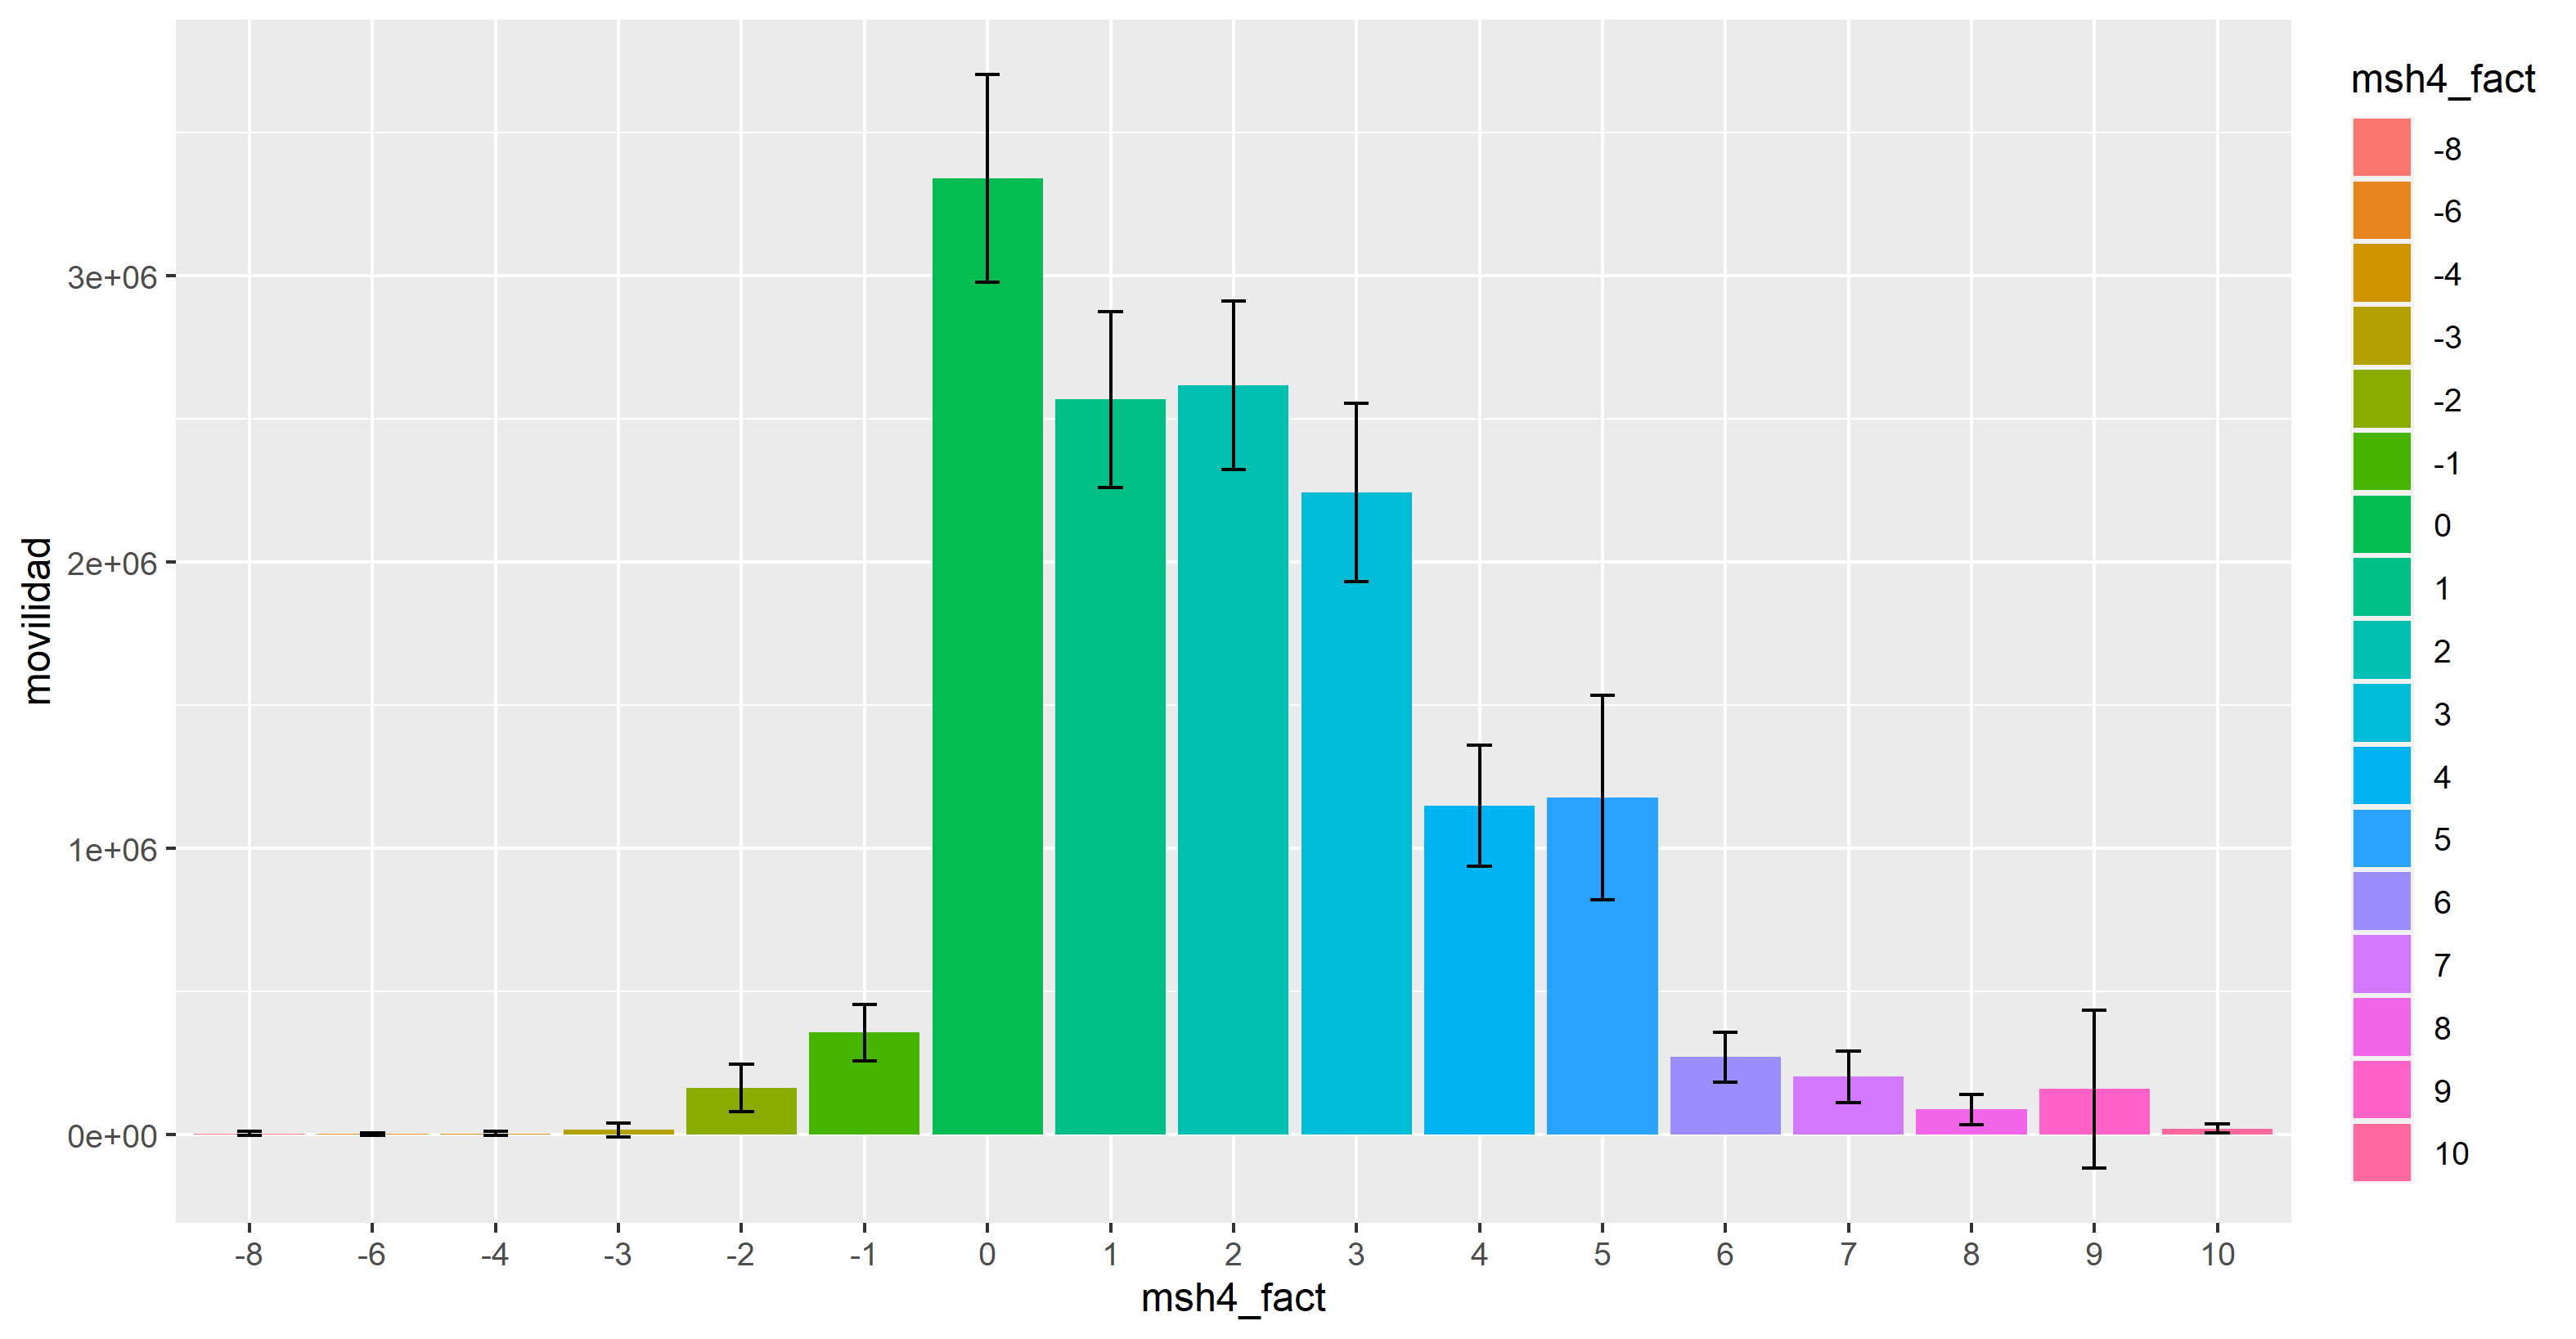
\includegraphics[width=0.8\linewidth,height=0.8\textheight]{output/graphs/graf2_exp} 

}

\caption{Movilidad social subjetiva esperada (población)}\label{fig:unnamed-chunk-10}
\end{figure}

Como se muestra en la figura 5, estos resultados también son
extrapolables a la población. Así, más de tres millones de habitantes
esperan que sus hijos ocupen la misma posición de la escala de estatus
social subjetivo en la que ellos se encuentran. Asimismo, un aproximado
de 7.5 millones de personas esperan que sus hijos se encuentren de una a
tres posiciones sobre la posición que ocupan ellos actualmente y cerca
de dos millones esperan que estén cuatro o cinco posiciones más arriba.
Sin embargo, aproximadamente 500mil habitantes esperan que sus hijos
experimenten una movilidad social subjetiva descendente.

\hypertarget{anuxe1lisis-bivariado}{%
\section{Análisis bivariado}\label{anuxe1lisis-bivariado}}

\begin{figure}

{\centering 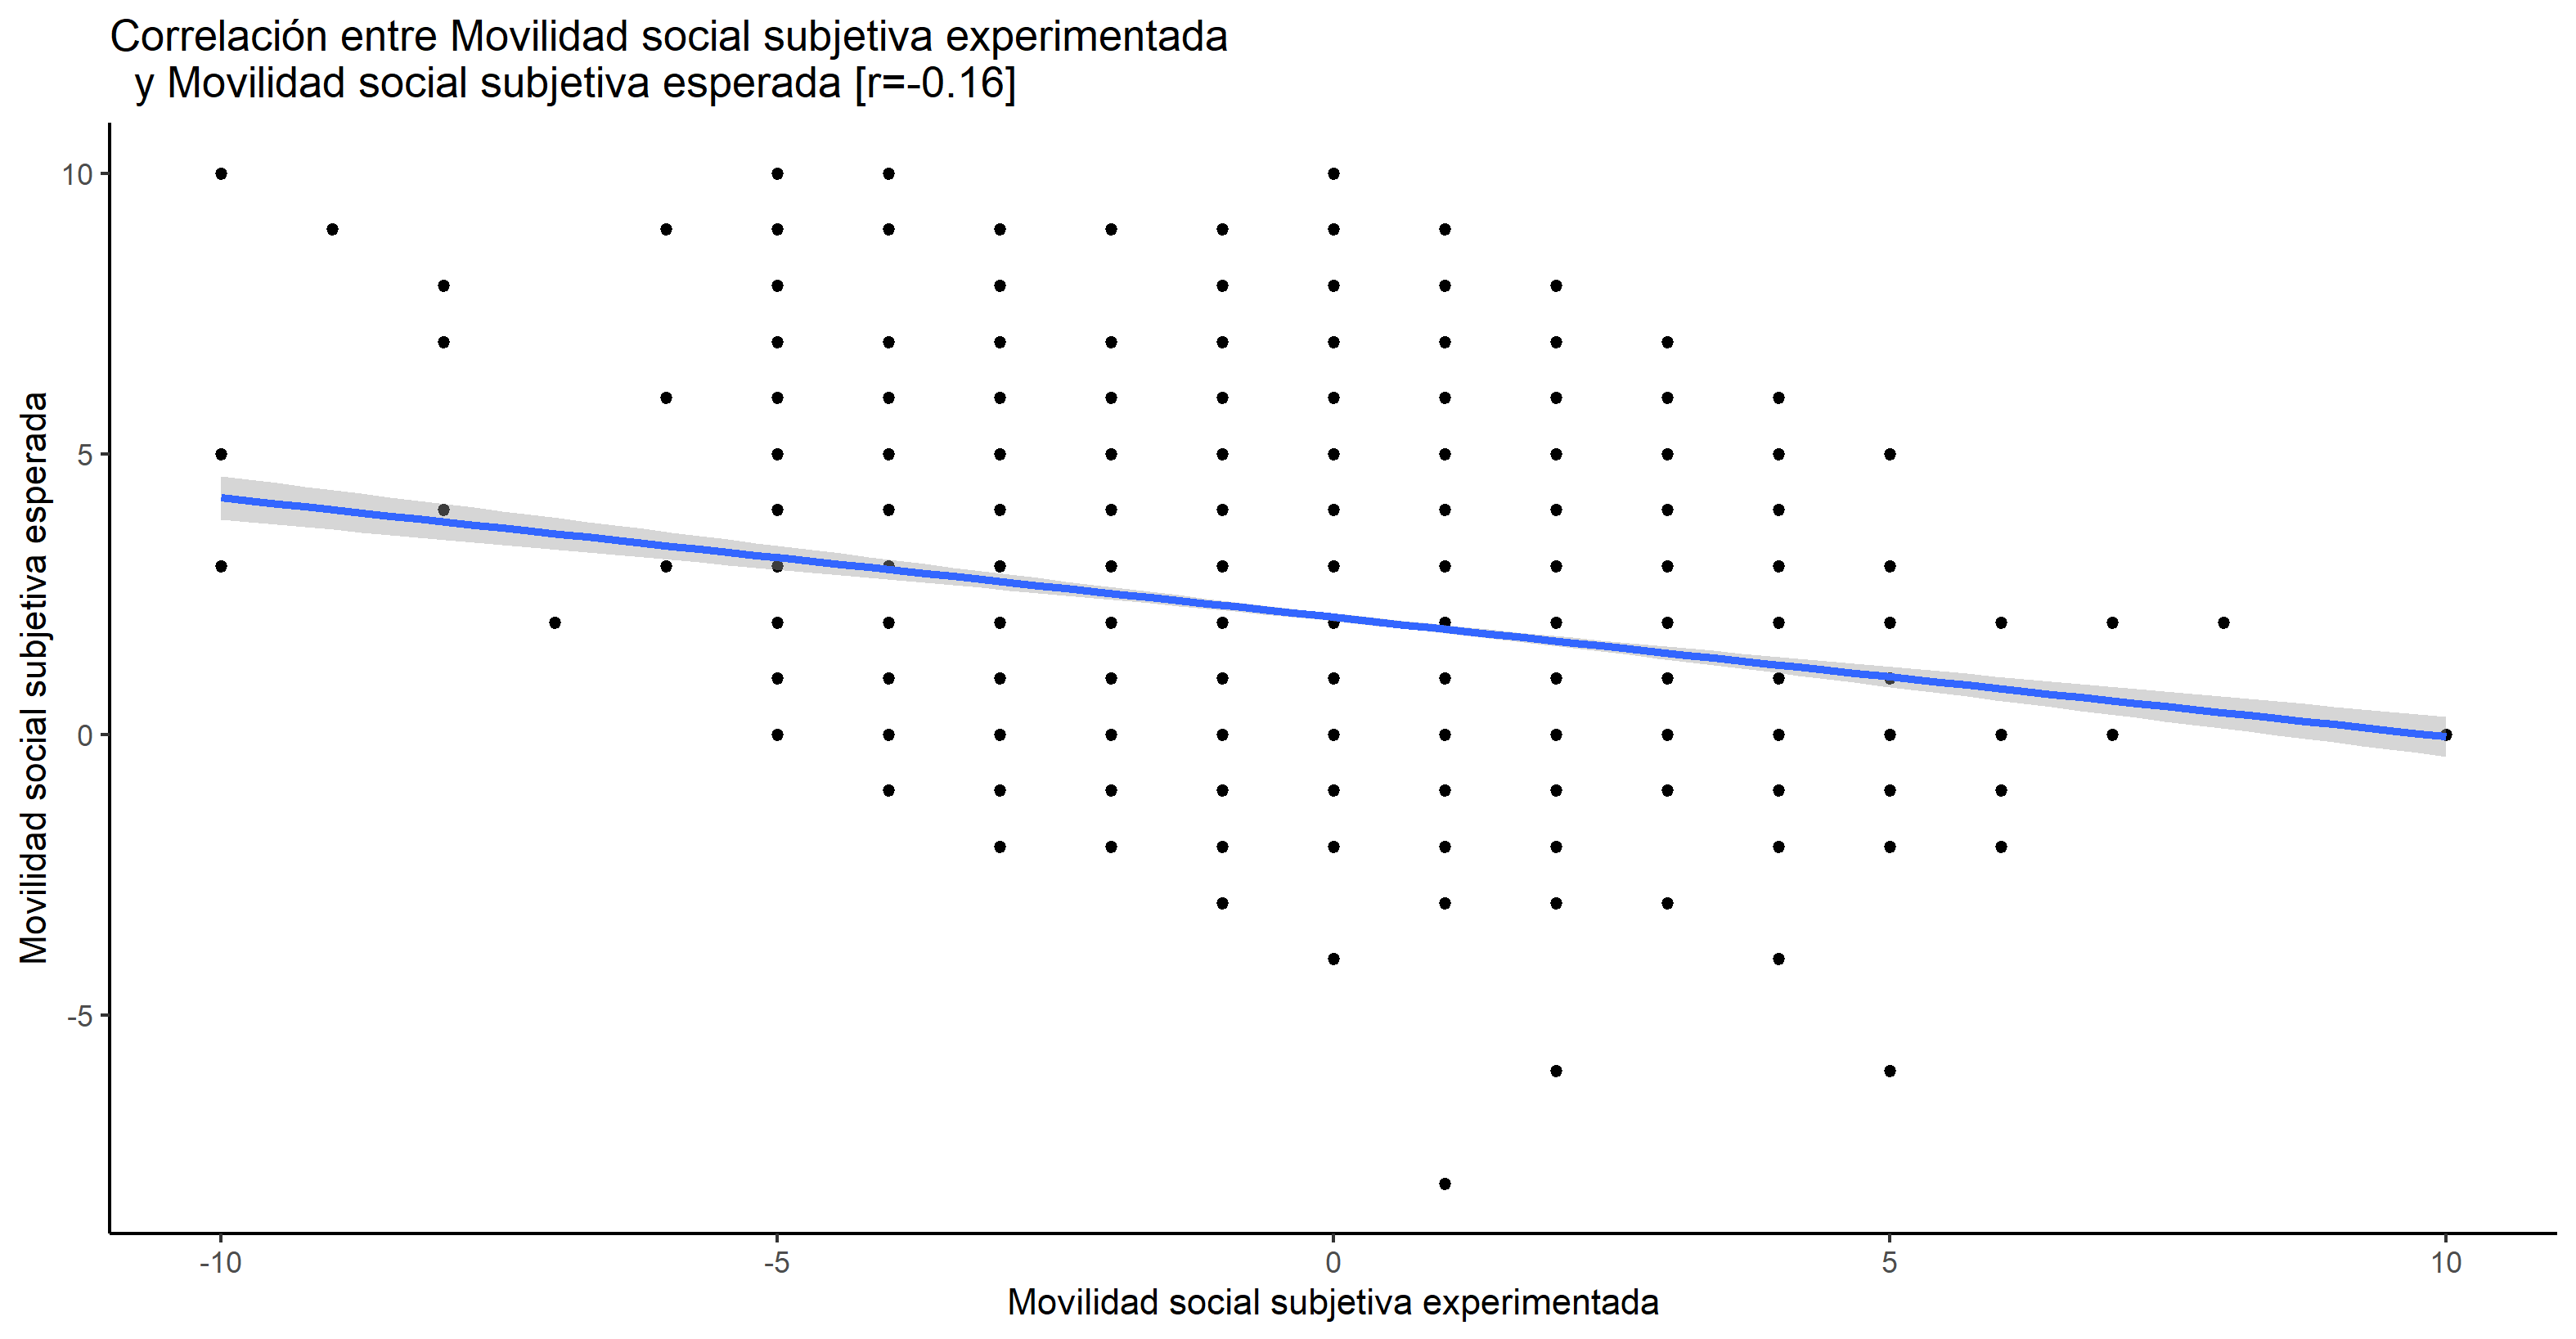
\includegraphics[width=0.8\linewidth,height=0.8\textheight]{output/graphs/graf8} 

}

\caption{Correlación entre movilidad social subjetiva experimentada y esperada}\label{fig:unnamed-chunk-11}
\end{figure}

En la figura 6 se muestra la correlación entre movilidad social
subjetiva experimentada y movilidad social subjetiva esperada. Como
ambas variables son ordinales, se estimó una correlación policórica que
posee un tamaño de r=-0.16. Al ser negativa, esta correlación indica
que, a medida que aumenta la Movilidad social subjetiva experimentada,
la movilidad social subjetiva esperada disminuye. Por lo tanto, la
percepción de experimentar un ascenso en la escala de estatus social
subjetivo implica que se espera que sus hijos no asciendan de la misma
forma o que desciendan en la escala de estatus social subjetivo.

\begin{figure}

{\centering 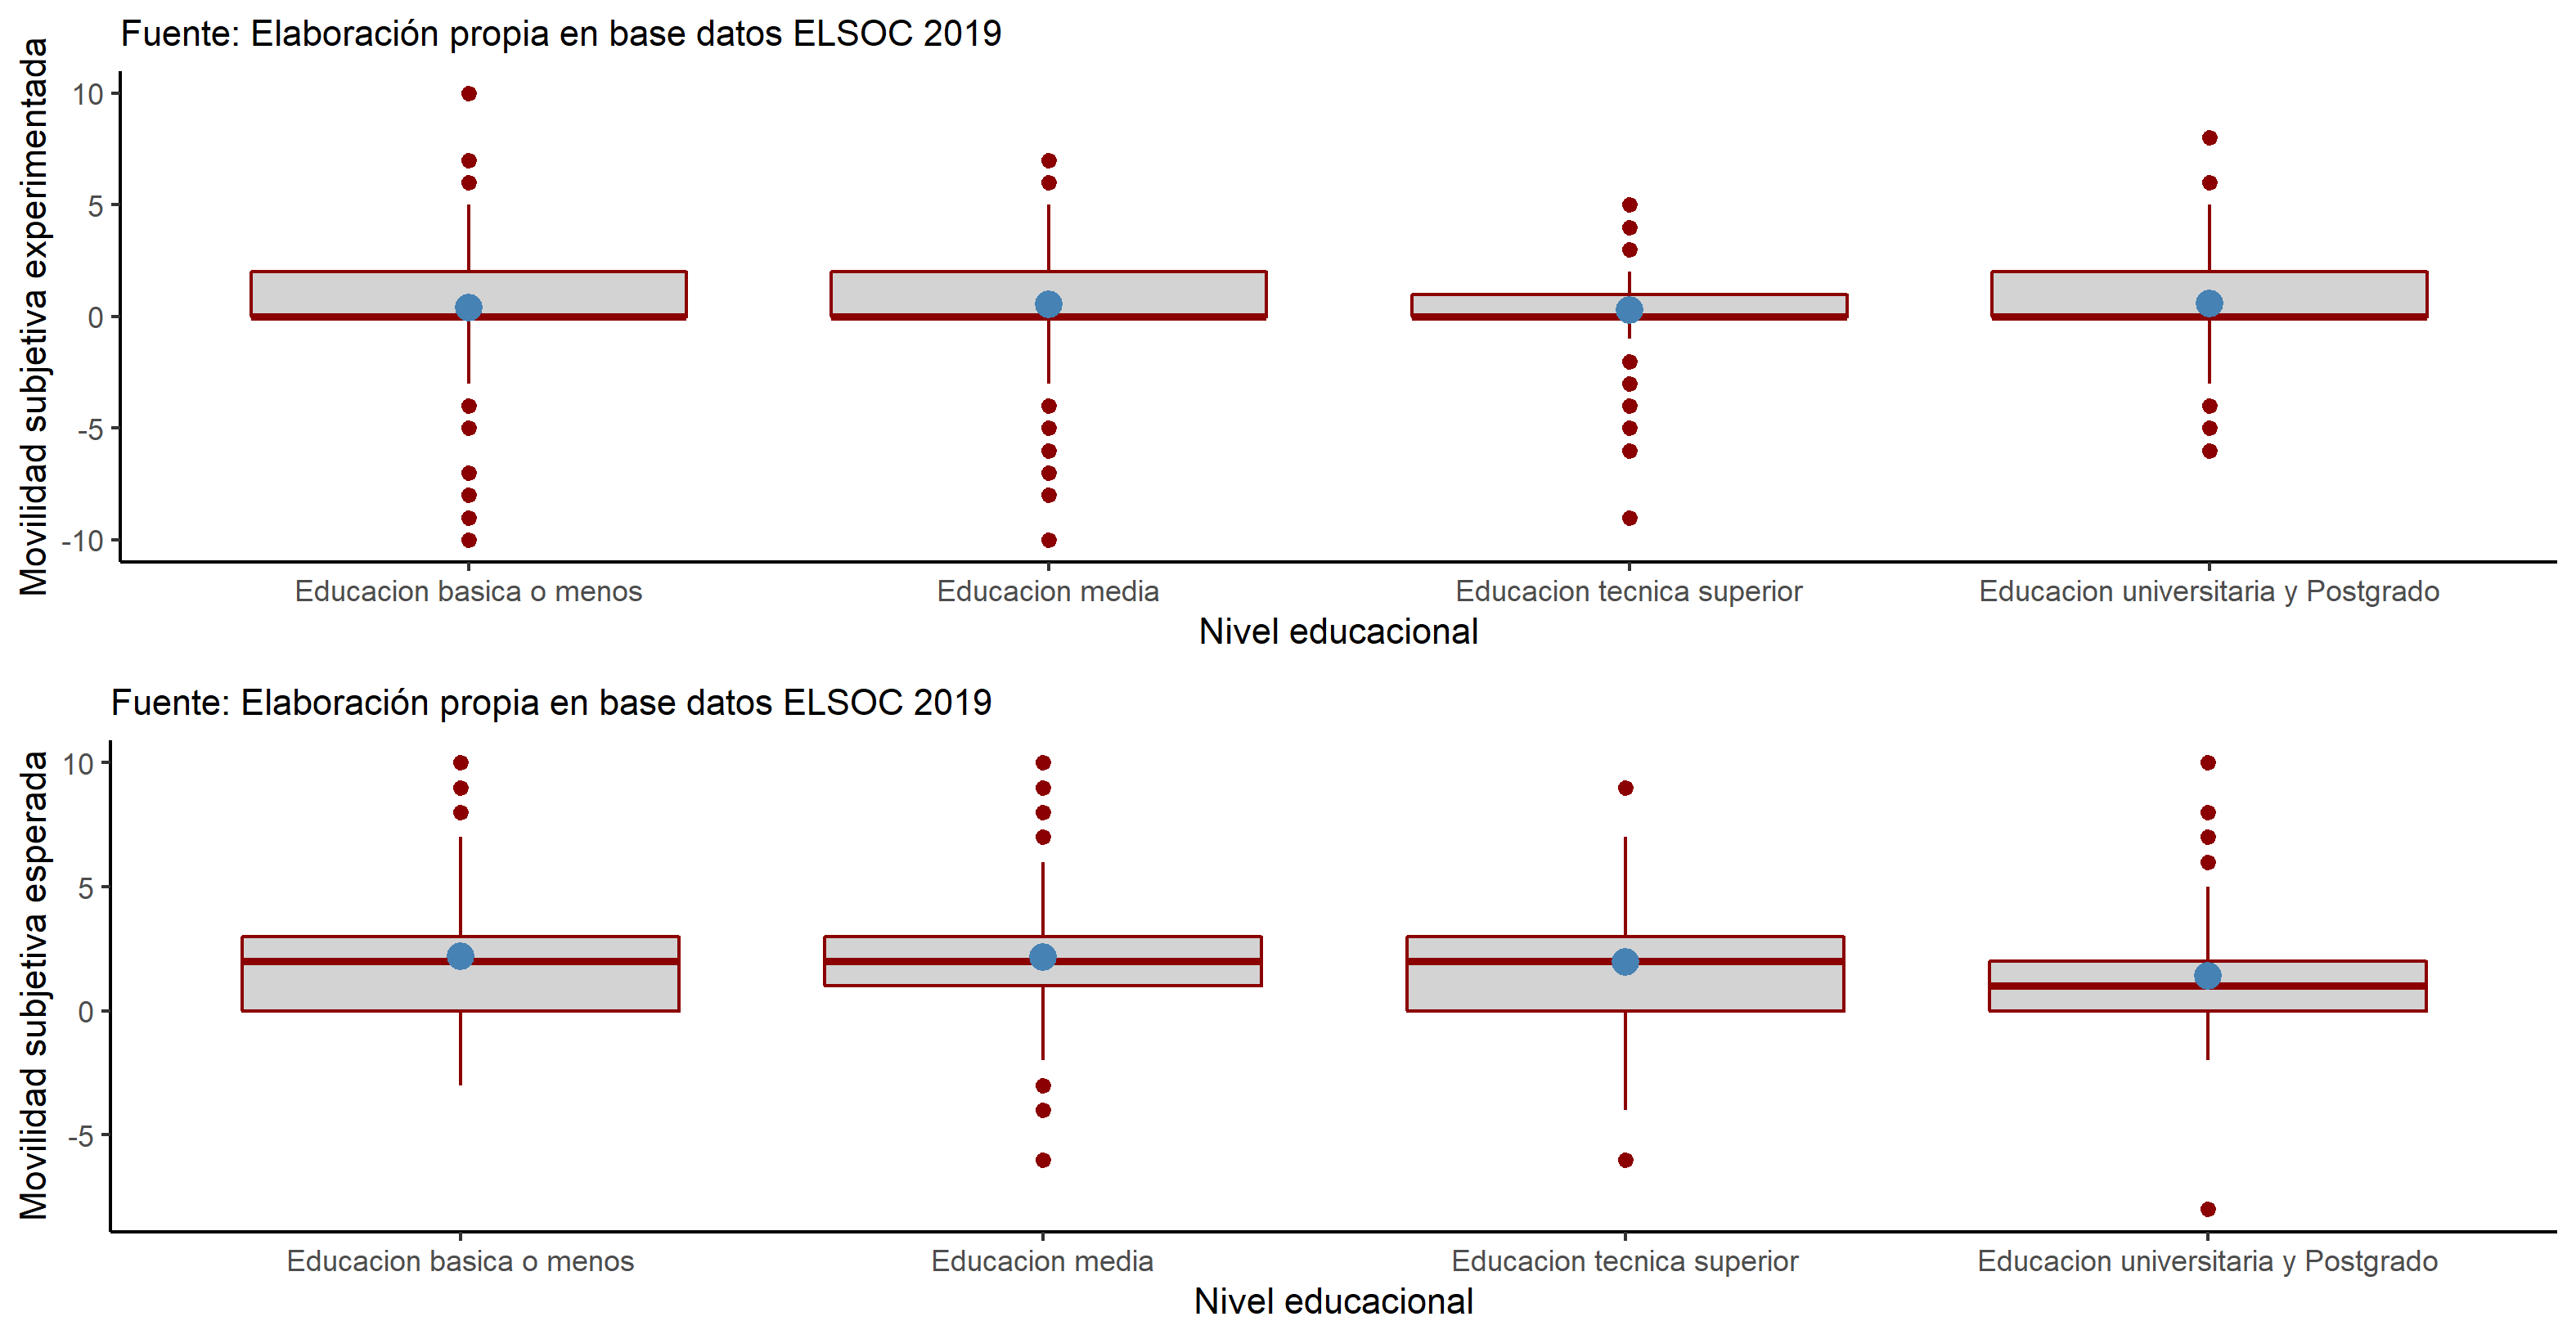
\includegraphics[width=1\linewidth,height=1\textheight]{output/graphs/graf3y4} 

}

\caption{Movilidad social subjetiva según nivel educacional}\label{fig:unnamed-chunk-12}
\end{figure}

En la figura 7 se presenta la percepción de movilidad social subjetiva
experimentada y esperada según el nivel educacional alcanzado. En
general, no se observan diferencias relevantes entre los grupos
educacionales para ninguna de las dos variables dependientes. Por un
lado, en relación con la movilidad social subjetiva experimentada, se
puede observar que para los cuatro niveles educacionales la mediana es 0
y su media es cercana a 0 (0.4 aproximadamente). Por otro lado, en
relación con la movilidad social subjetiva esperada, tres de los cuatro
grupos poseen una media de 2.6 y una mediana de 2.5, mientras que
quienes poseen educación universitaria o postgrado tienen una mediana de
2 y una media de 2.5.

\begin{figure}

{\centering 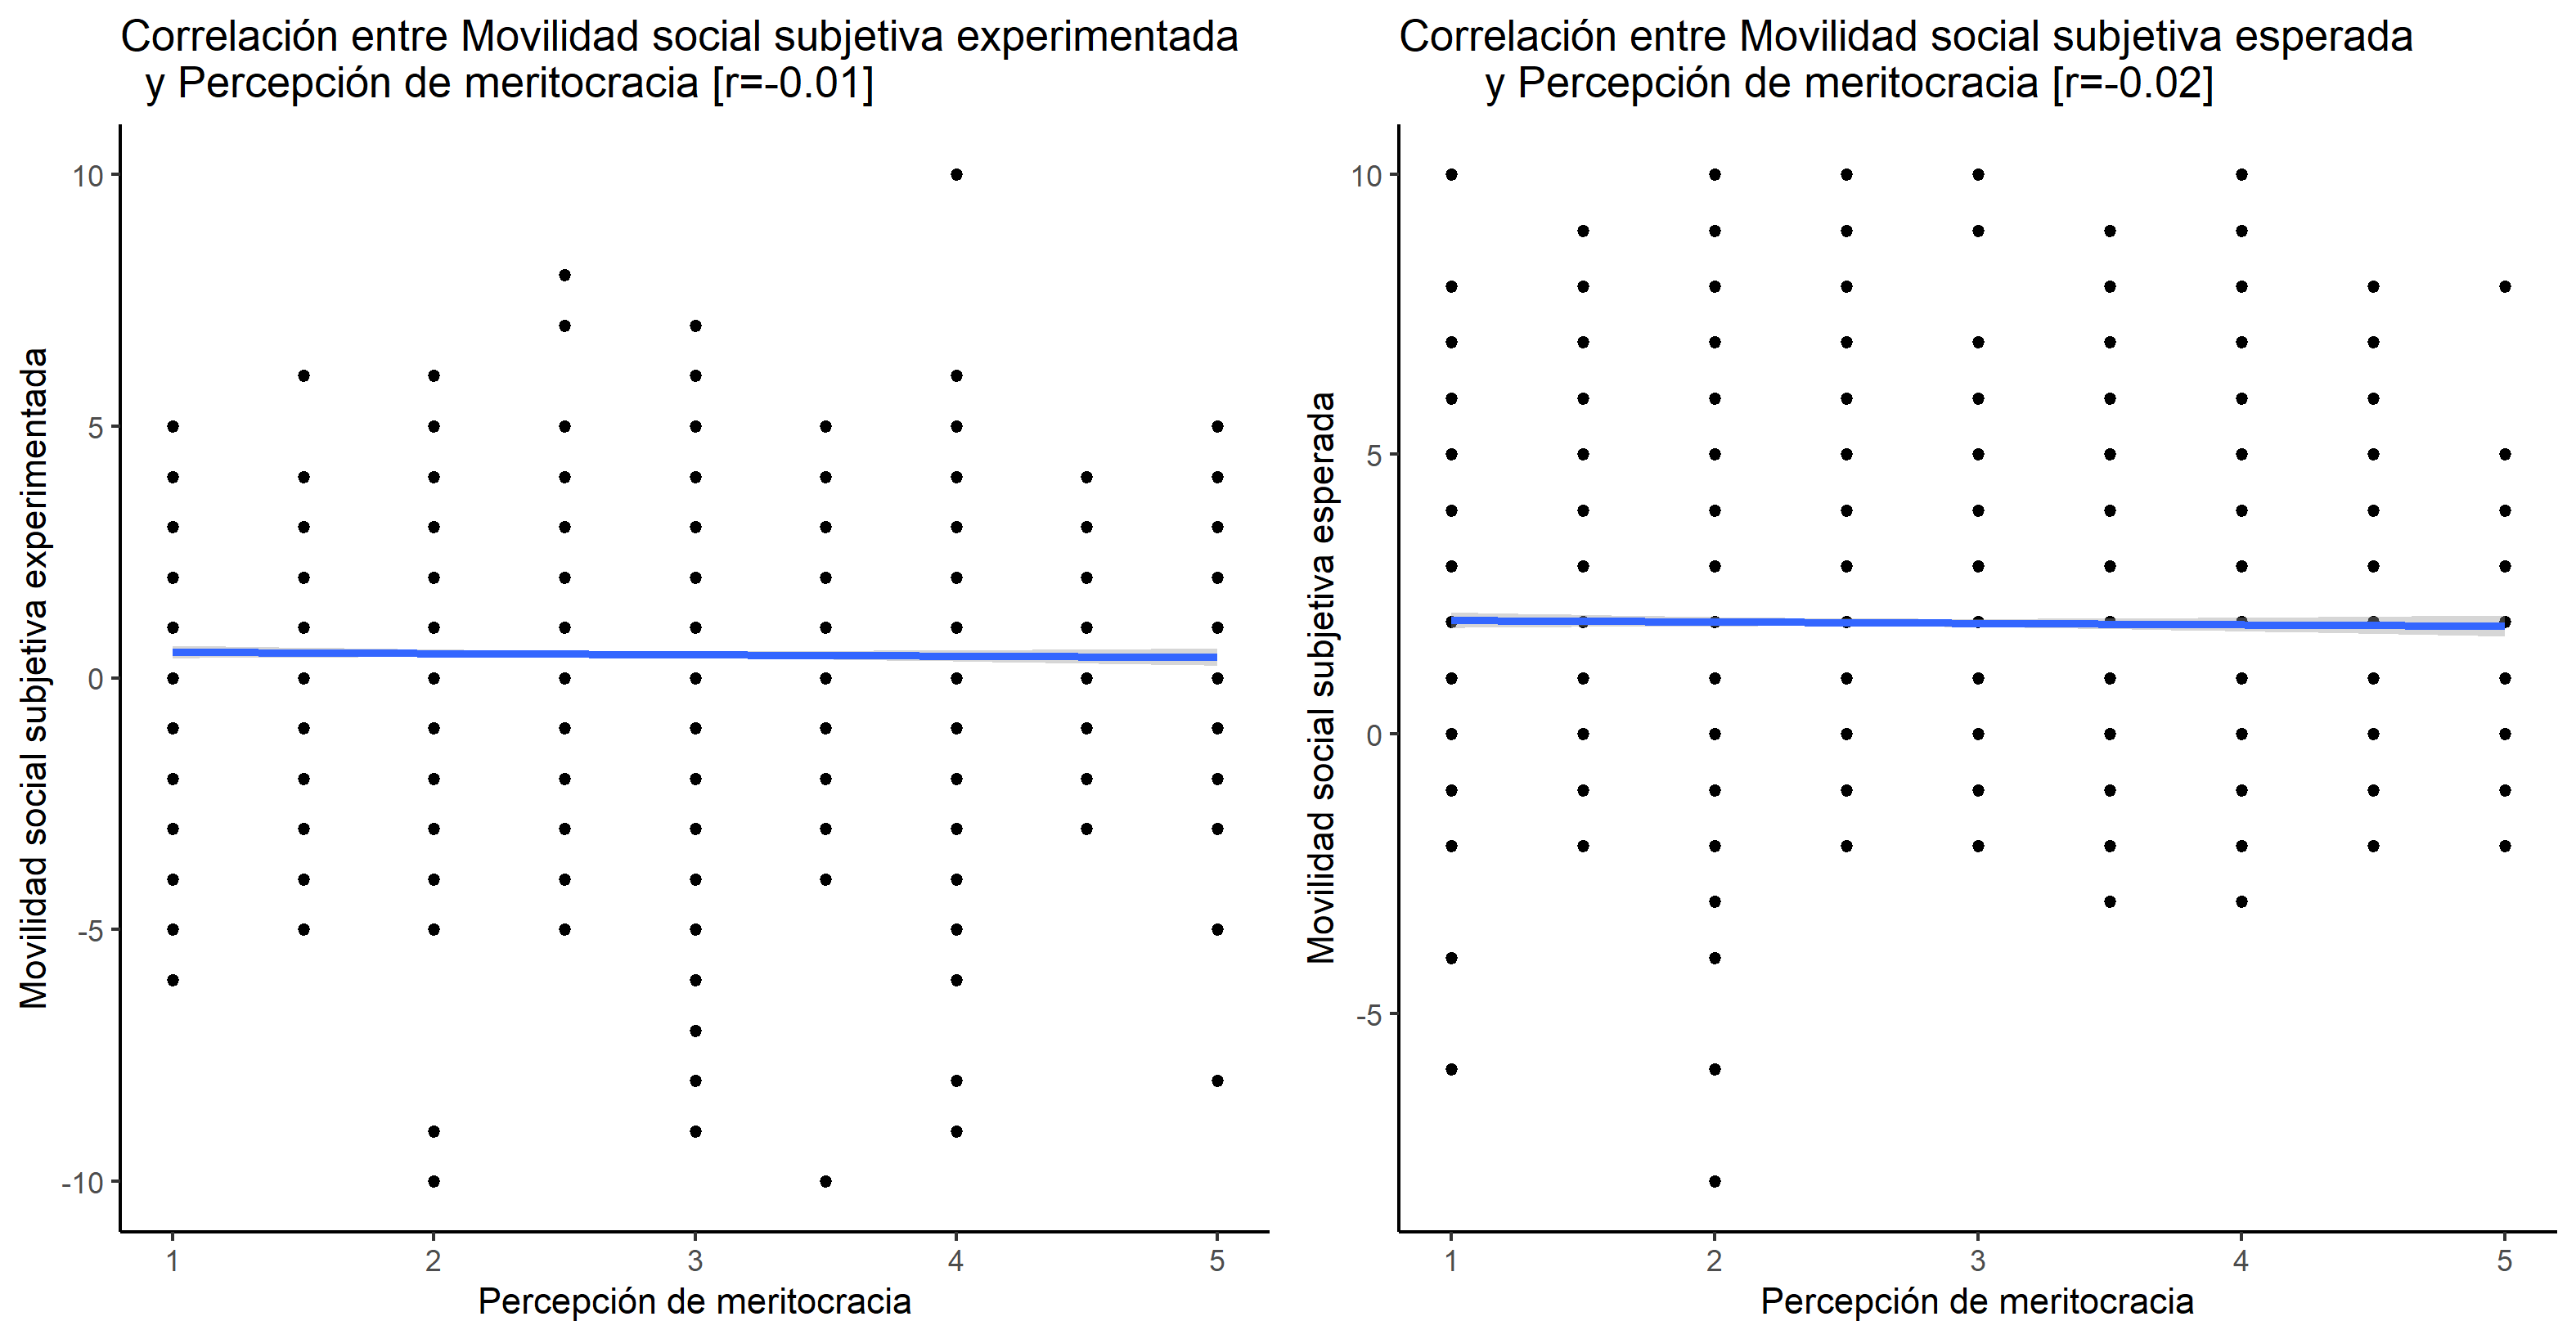
\includegraphics[width=1\linewidth,height=1\textheight]{output/graphs/graf6y7} 

}

\caption{Correlación entre movilidad social subjetiva y percepción de meritocracia}\label{fig:unnamed-chunk-13}
\end{figure}

En la figura 8 se presenta la correlación que existe entre la percepción
de movilidad social subjetiva experimentada y esperada y la percepción
de meritocracia. Al tratarse de variables ordinales, se estimaron
correlaciones policóricas, las que poseen un tamaño de r=-0.01 para la
movilidad subjetiva experimentada y de r=-0.02 para la movilidad
subjetiva esperada. En este sentido, estas correlaciones poseen una
dirección negativa, en el sentido de que, a medida que aumenta la
percepción de meritocracia, la percepción de movilidad social subjetiva
disminuye. Sin embargo, la fuerza de esta correlación es casi nula, por
lo que no se puede concluir que la percepción de meritocracia influya de
manera importante en la percepción de movilidad social subjetiva.

\newpage

\hypertarget{conclusiones}{%
\section{Conclusiones}\label{conclusiones}}

A partir de los resultados presentados es posible señalar que se cumple
lo planteado por investigaciones previas: la percepción de movilidad
social subjetiva -al igual que la movilidad social ocupacional y la
movilidad educacional- da cuenta de una estructura social rígida. En
este sentido, las hipótesis 1 y 2 se cumplen parcialmente. Los
resultados muestran que la mayoría de la población percibe que se
encuentra en la misma posición de la escala de estatus social subjetivo
que sus padres y que, además, sus hijos también estarán en esta misma
posición. Asimismo, si bien se percibe que se ha experimentado un
ascenso antes que un descenso en la escala de estatus social subjetivo,
la mayoría de la población percibe que ha ascendido solo una o dos
posiciones y espera que sus hijos asciendan de una a cuatro posiciones
en la escala de estatus social subjetivo. Por lo tanto, de cierta forma
se cumple lo señalado por Espinoza, et. al
(\protect\hyperlink{ref-espinoza_Estratificacion_2013}{2013}) sobre que
hay una estructura de clases relativamente móvil y permeable pero solo
en su parte media, a la vez que las distancias sociales entre quienes
ocupan las posiciones altas de la sociedad y quienes se encuentran más
abajo siguen aumentando. En términos concretos, esto representa que en
Chile existe una baja movilidad intergeneracional percibida, ya que la
posición social de las personas se ve determinada por la posición social
de sus padres.

En cuanto a la tercera hipótesis, no se encuentra evidencia que la
sustente, ya que la percepción de una experiencia de ascenso en la
escala de estatus social subjetivo no se asocia con un aprendizaje que
podría traducirse en una esperanza de ascenso para los hijos. Por el
contrario, un mayor grado de movilidad social subjetiva experimentada se
asocia con menores niveles de movilidad social subjetiva esperada. Esto
implica que, incluso entre quienes perciben que han experimentado una
movilidad social subjetiva ascendente, no se espera que sus hijos tengan
mejores oportunidades y que asciendan en la escala de estatus social
subjetivo.

En relación con las hipótesis 4.1 y 4.2, al abordar aspectos objetivos y
subjetivos que podrían afectar la percepción de movilidad social
subjetiva experimentada y esperada no se encontraron nuevos resultados
que sustenten las evidencias previas. Alcanzar un mayor nivel
educacional no implica diferencias en la percepción de movilidad social
subjetiva, así como tampoco lo hace una mayor percepción de
meritocracia. De esta forma, más allá de los sesgos que puedan existir
por las diferencias de origen social o de creencias culturales, la
percepción de movilidad social es la misma.

En cuanto a este último término, una de las limitantes de este estudio
es la forma en que fue construida la variable dependiente y que podrían
influir en los efectos que tengan los factores objetivos y subjetivos
sobre ella. Es decir, una persona que ha experimentado una gran
movilidad social subjetiva ascendente de, por ejemplo, 8 unidades, no
podría esperar que sus hijos asciendan en la misma magnitud en la escala
de estatus social subjetivo (si asciende 8 unidades, solo deja un margen
de 2 unidades por ascender). Por lo que existe un cierto margen de
variabilidad que este indicador no logra capturar.

Sin embargo, a pesar de esta limitante, es necesario continuar con este
tipo de investigaciones que intentan analizar la forma en que las
personas perciben las oportunidades que brinda cada sociedad, ya sea a
través de nuevos indicadores que aborden movilidad social subjetiva o a
través de otros factores objetivos o subjetivos que podrían influir en
las percepciones de los individuos. En este sentido, en la sociedad
chilena existen características adscriptivas que podrían estar asociadas
a la percepción de movilidad social subjetiva, como lo son el sexo, la
raza o la condición de inmigración.

\newpage

\hypertarget{referencias}{%
\section{Referencias}\label{referencias}}

\hypertarget{refs}{}
\leavevmode\hypertarget{ref-benabou_Social_1998}{}%
Benabou, R., \& Ok, E. (1998). \emph{Social Mobility and the Demand for
Redistribution: The POUM Hypothesis} (Nos. w6795; p. w6795). National
Bureau of Economic Research. \url{https://doi.org/10.3386/w6795}

\leavevmode\hypertarget{ref-castillo_Meritocracia_2019}{}%
Castillo, J. C., Torres, A., Atria, J., \& Maldonado, L. (2019).
Meritocracia y desigualdad económica: Percepciones, preferencias e
implicancias. \emph{Revista Internacional de Sociología}, \emph{77}(1),
117. \url{https://doi.org/10.3989/ris.2019.77.1.17.114}

\leavevmode\hypertarget{ref-castillo_Educacion_2013}{}%
Castillo, J., Madero-Cabib, I., \& Miranda, D. (2013). Educación,
equidad y creencias distributivas: Evidencias del caso chileno.
\emph{Sociedad Hoy}, \emph{24}, 13--31.

\leavevmode\hypertarget{ref-castillo_Todos_2013}{}%
Castillo, Miranda, \& Madero-Cabib. (2013). Todos Somos Clase Media:
Sobre el estatus social subjetivo en Chile. \emph{Latin American
Research Review}, \emph{48}(01), 155--173.

\leavevmode\hypertarget{ref-cepal_hora_2010}{}%
CEPAL. (2010). \emph{La hora de la igualdad: Brechas por cerrar, caminos
por abrir. Trigésimo Tercer Período de Sesiones de la CEPAL}.

\leavevmode\hypertarget{ref-coes_Radiografia_2019}{}%
COES. (2019). \emph{Radiografía del cambio social. Análisis de
Resultados Longitudinales 2016-2018}.

\leavevmode\hypertarget{ref-coes_Estudio_2021}{}%
COES. (2021). \emph{Estudio Longitudinal Social de Chile -
https://coes.cl/encuesta-panel/}.

\leavevmode\hypertarget{ref-espinoza_Estratificacion_2013}{}%
Espinoza, V., Barozet, E., \& Méndez, M. L. (2013). Estratificación y
movilidad social bajo un modelo neoliberal: El caso de Chile.
\emph{Lavboratorio}, \emph{25}, 169--191.

\leavevmode\hypertarget{ref-gavira_Social_2008}{}%
Gavira, A. (2008). Social Mobility and Preferences for Redistribution in
Latin America. \emph{Economía}, \emph{8}(1), 55--88.
\url{https://doi.org/10.1353/eco.2008.0003}

\leavevmode\hypertarget{ref-huang_Effects_2017}{}%
Huang, S., Hou, J., Sun, L., Dou, D., Liu, X., \& Zhang, H. (2017). The
Effects of Objective and Subjective Socioeconomic Status on Subjective
Well-Being among Rural-to-Urban Migrants in China: The Moderating Role
of Subjective Social Mobility. \emph{Frontiers in Psychology}, \emph{8},
819. \url{https://doi.org/10.3389/fpsyg.2017.00819}

\leavevmode\hypertarget{ref-perezverdugo_Factores_2018}{}%
Pérez Verdugo, C. (2018). \emph{Factores socioeconómicos que influyen en
la legitimación de la desigualdad en educación}.
\url{https://doi.org/10.13140/RG.2.2.17256.62728}

\leavevmode\hypertarget{ref-pnud_Desiguales_2017}{}%
PNUD (Ed.). (2017). \emph{Desiguales: Orígenes, cambios y desafíos de la
brecha social en Chile}. PNUD : Uqbar Editores.

\leavevmode\hypertarget{ref-prag_Subjective_2021}{}%
Präg, P., \& Gugushvili, A. (2021). Subjective social mobility and
health in Germany. \emph{European Societies}, 1--23.
\url{https://doi.org/10.1080/14616696.2021.1887916}

\leavevmode\hypertarget{ref-ruiz_chilenos_2014}{}%
Ruiz, C., \& Boccardo, G. (2014). \emph{Los chilenos bajo el
neoliberalismo: Clases y conflicto social} (Primera edición). Ediciones
y Publicaciones El Buen Aire.

\leavevmode\hypertarget{ref-torche_Estratificacion_2004}{}%
Torche, F., \& Wormald, G. (2004). \emph{Estratificación y movilidad
social en Chile: entre la adscripción y el logro}. Naciones Unidas,
CEPAL, División de Desarrollo Social.

\leavevmode\hypertarget{ref-zhang_Family_2021}{}%
Zhang, F., Jiang, Y., Huang, S., Ming, H., Ren, Y., \& Wang, L. (2021).
Family Socioeconomic Status, Parental Involvement, and Academic
Achievement: The Moderating Role of Adolescents' Subjective Social
Mobility. \emph{The Journal of Early Adolescence}, 027243162110022.
\url{https://doi.org/10.1177/02724316211002254}

\end{document}
